%% Author:	Frank Berghaus modified by Chris Geroux
%% File:	draft2.tex
%% Date:	24.07.2003
%% Purpose:	Undergrad Thesis.

\documentclass[12pt, oneside]{smuthesis}
\input{epsf}
%---> SET UP MARGINS <--------------------------------------------------------------------
% original margin settings
%\setlength{\textwidth}{16.5cm}
%\setlength{\oddsidemargin}{1.0cm}
%\setlength{\evensidemargin}{1.0cm}
%\setlength{\topmargin}{-2.0cm}
%\setlength{\textheight}{23.5cm}
%
% Brynle's revised margin settings
\setlength{\textwidth}      {6.0in}   % sets text width  = 6.0 in
\setlength{\textheight}     {9.0in}   % sets text height = 9.0 in
\setlength{\topmargin}      {-0.25in} % sets top  margin = 1.0 in
\setlength{\evensidemargin} {0.485in} % sets left margin = 1.5 in
\setlength{\oddsidemargin}  {0.485in} % sets left margin = 1.5 in
\setlength{\footskip}       {1.0in}   % allows up to 1.0 in for footers
%
%---> PACKAGES <--------------------------------------------------------------------------
\usepackage{psfigure}
\usepackage{latexsym,multicol,epsfig}
\usepackage{setspace}
%\usepackage{supertabular}
\usepackage{multirow}
\usepackage{booktabs}
\usepackage{alltt}
\usepackage{graphicx}
\usepackage{caption}
\usepackage{subcaption}
\usepackage{amsmath}
\usepackage{amssymb}
\usepackage[round]{natbib}
\usepackage{indentfirst}
\usepackage{float}
\usepackage{harpoon}
\usepackage{fancyvrb}
\usepackage{stackengine}
\usepackage{calc}
\newlength\shlength
\newcommand\xshlonghvecr[2][1]{\setlength\shlength{#1pt}%
	\stackengine{-1.0pt}{$#2$}{\smash{$\kern\shlength%
			\stackengine{2.75pt}{$\mathchar"012A$}%
			{\rule{\widthof{$#2$}}{.50pt}\kern1pt}{O}{r}{F}{F}{L}\kern-\shlength$}}%
	{O}{c}{F}{T}{S}}
\newcommand\xshlonghvecl[2][1]{\setlength\shlength{#1pt}%
	\stackengine{-1.0pt}{$#2$}{\smash{$\kern\shlength%
			\stackengine{2.75pt}{\kern-1pt$\mathchar"0128$}%
			{\rule{\widthof{$#2$}}{.50pt}\kern1pt}{O}{l}{F}{F}{L}\kern-\shlength$}}%
	{O}{c}{F}{T}{S}}
\newcommand{\mixtensor}[3]{{#1}^{#2}{}_{#3}}
\newcommand{\contensor}[2]{{#1}^{#2}}
\newcommand{\covtensor}[2]{{#1}_{#2}}
%---> Resource Directories <----------------------------------------------------
% Images
\graphicspath{{./img/}}

\bibliographystyle{plainnat}
\newcommand{\code}[1]{\texttt{#1}}%allows \code{stuff} to be \textt{stuff} used for code varibles
\newcommand{\dd}[1]{\mathrm{d}#1}
%
%---> TITLE PAGE <------------------------------------------------------------------------
\def\figurebox#1#2#3{%
    \def\arg{#3}%
    \ifx\arg\empty
    {\hfill\vbox{\hsize#2\hrule\hbox to #2{\vrule\hfill\vbox to #1{\hsize#2%
     \vfill}\vrule}\hrule}\hfill}%
    \else
    {\hfill\epsfbox{#3}\hfill}%
    \fi}
\degreetitle{Bachelor of Science}
\numberofsignatures{5}
%
%---> Define Variables such as title etc <------------------------------------------------
\newcommand{\myTitle}{Investigating Supermassive Black Holes and their variability by using a Structure Function}
%
%---> BEGIN DOCUMENT <--------------------------------------------------------------------
\begin{document}
\frontmatter
%---> TITLE <-----------------------------------------------------------------------------
\title{\sc \myTitle}
\author{Derek Blue}
\date{today}
\medskip

\maketitle
\pagestyle{headings}

%---> ABSTRACT <--------------------------------------------------------------------------
%% Apparently they want the title and name of the author in the abstract ...
\begin{center}
\section*{\center \sc Abstract} \label{abstract}
\sc \myTitle
\paragraph*{\center  \\}
\end{center}
Viewed from Earth, regardless of the direction one looks, our universe is populated with galaxies as far as we can currently observer. The currently accepted theoretical model is that supermassive black holes reside at the center of galaxies. This has been proven for a majority of observable galaxies, including our own. For some the central black hole is actively accreting matter and these galaxies are called active galaxies. Active galaxies are of particular interest because when viewed over the entire electromagnetic spectrum they are some of the brightest objects in the night sky. In addition, their emission spectra are incredibly variable. Unfortunately since the data acquired from these objects is generally unevenly sampled, a Fourier analysis cannot be used to investigate them as it suffers from windowing and aliasing. For these reasons a structure function was used, which provides similar information as the Fourier analysis, but with the added benefits of remaining in the time domain and sporting a robustness against windowing and aliasing due to uneven sampling.

\begin{center}
by {\em Derek Blue}\\
submitted on \today:\\
\end{center}
\newpage

%---> TABLE OF CONTENTS <----------------------------------------------------------------
\tableofcontents
\listoffigures
\listoftables
\newpage
%
%---> INTRODUCTION <---------------------------------------------------------------------
\mainmatter
\chapter{\sc Introduction} \label{introduction}

\section{\sc Overview} \label{overview}

This chapter will give an overview of the objects, theoretical models, and observation methods user in the rest of this work. The majority of this thesis is concerned with the analysis of the electromagnetic spectrum emitted by supermassive black holes at the centers of various galaxies. by using a structure function, which will be described in detail. This analysis was done in order to improve understanding of the theoretical model used to describe active galactic nuclei.

\section{\sc Galaxies} \label{galaxies}

We all learn from a young age that our planet Earth resides in a galaxy known as The Milky Way. But what is a galaxy?

Galaxies are relatively faint objects in comparison to stars when being observed with the naked eye. So it comes as no surprise that they were not discovered until telescope technology had advanced to a sufficient degree as to allow a significant enough amount of light in to view very distant objects. In 1845 William Parsons of Ireland, known better as Lord Ross, built a telescope that would be the largest of it's time, known as the Ross Telescope. In using this telescope he was able to observe groupings of stars and gas and dust distant from our own Milky Way that demonstrated a sort of spiral structure. Initially Parsons believed these to be nebulae but soon concluded that they were "great clouds of stars"\footnote{\cite{sag}} beyond our galaxy.

These great clouds of stars are now theorized by modern astronomers to contain supermassive black holes at their centers holding them together. Supermassive black holes, as their name suggests and as this chapter will explain later are extremely massive.

\begin{figure}
	\centering
	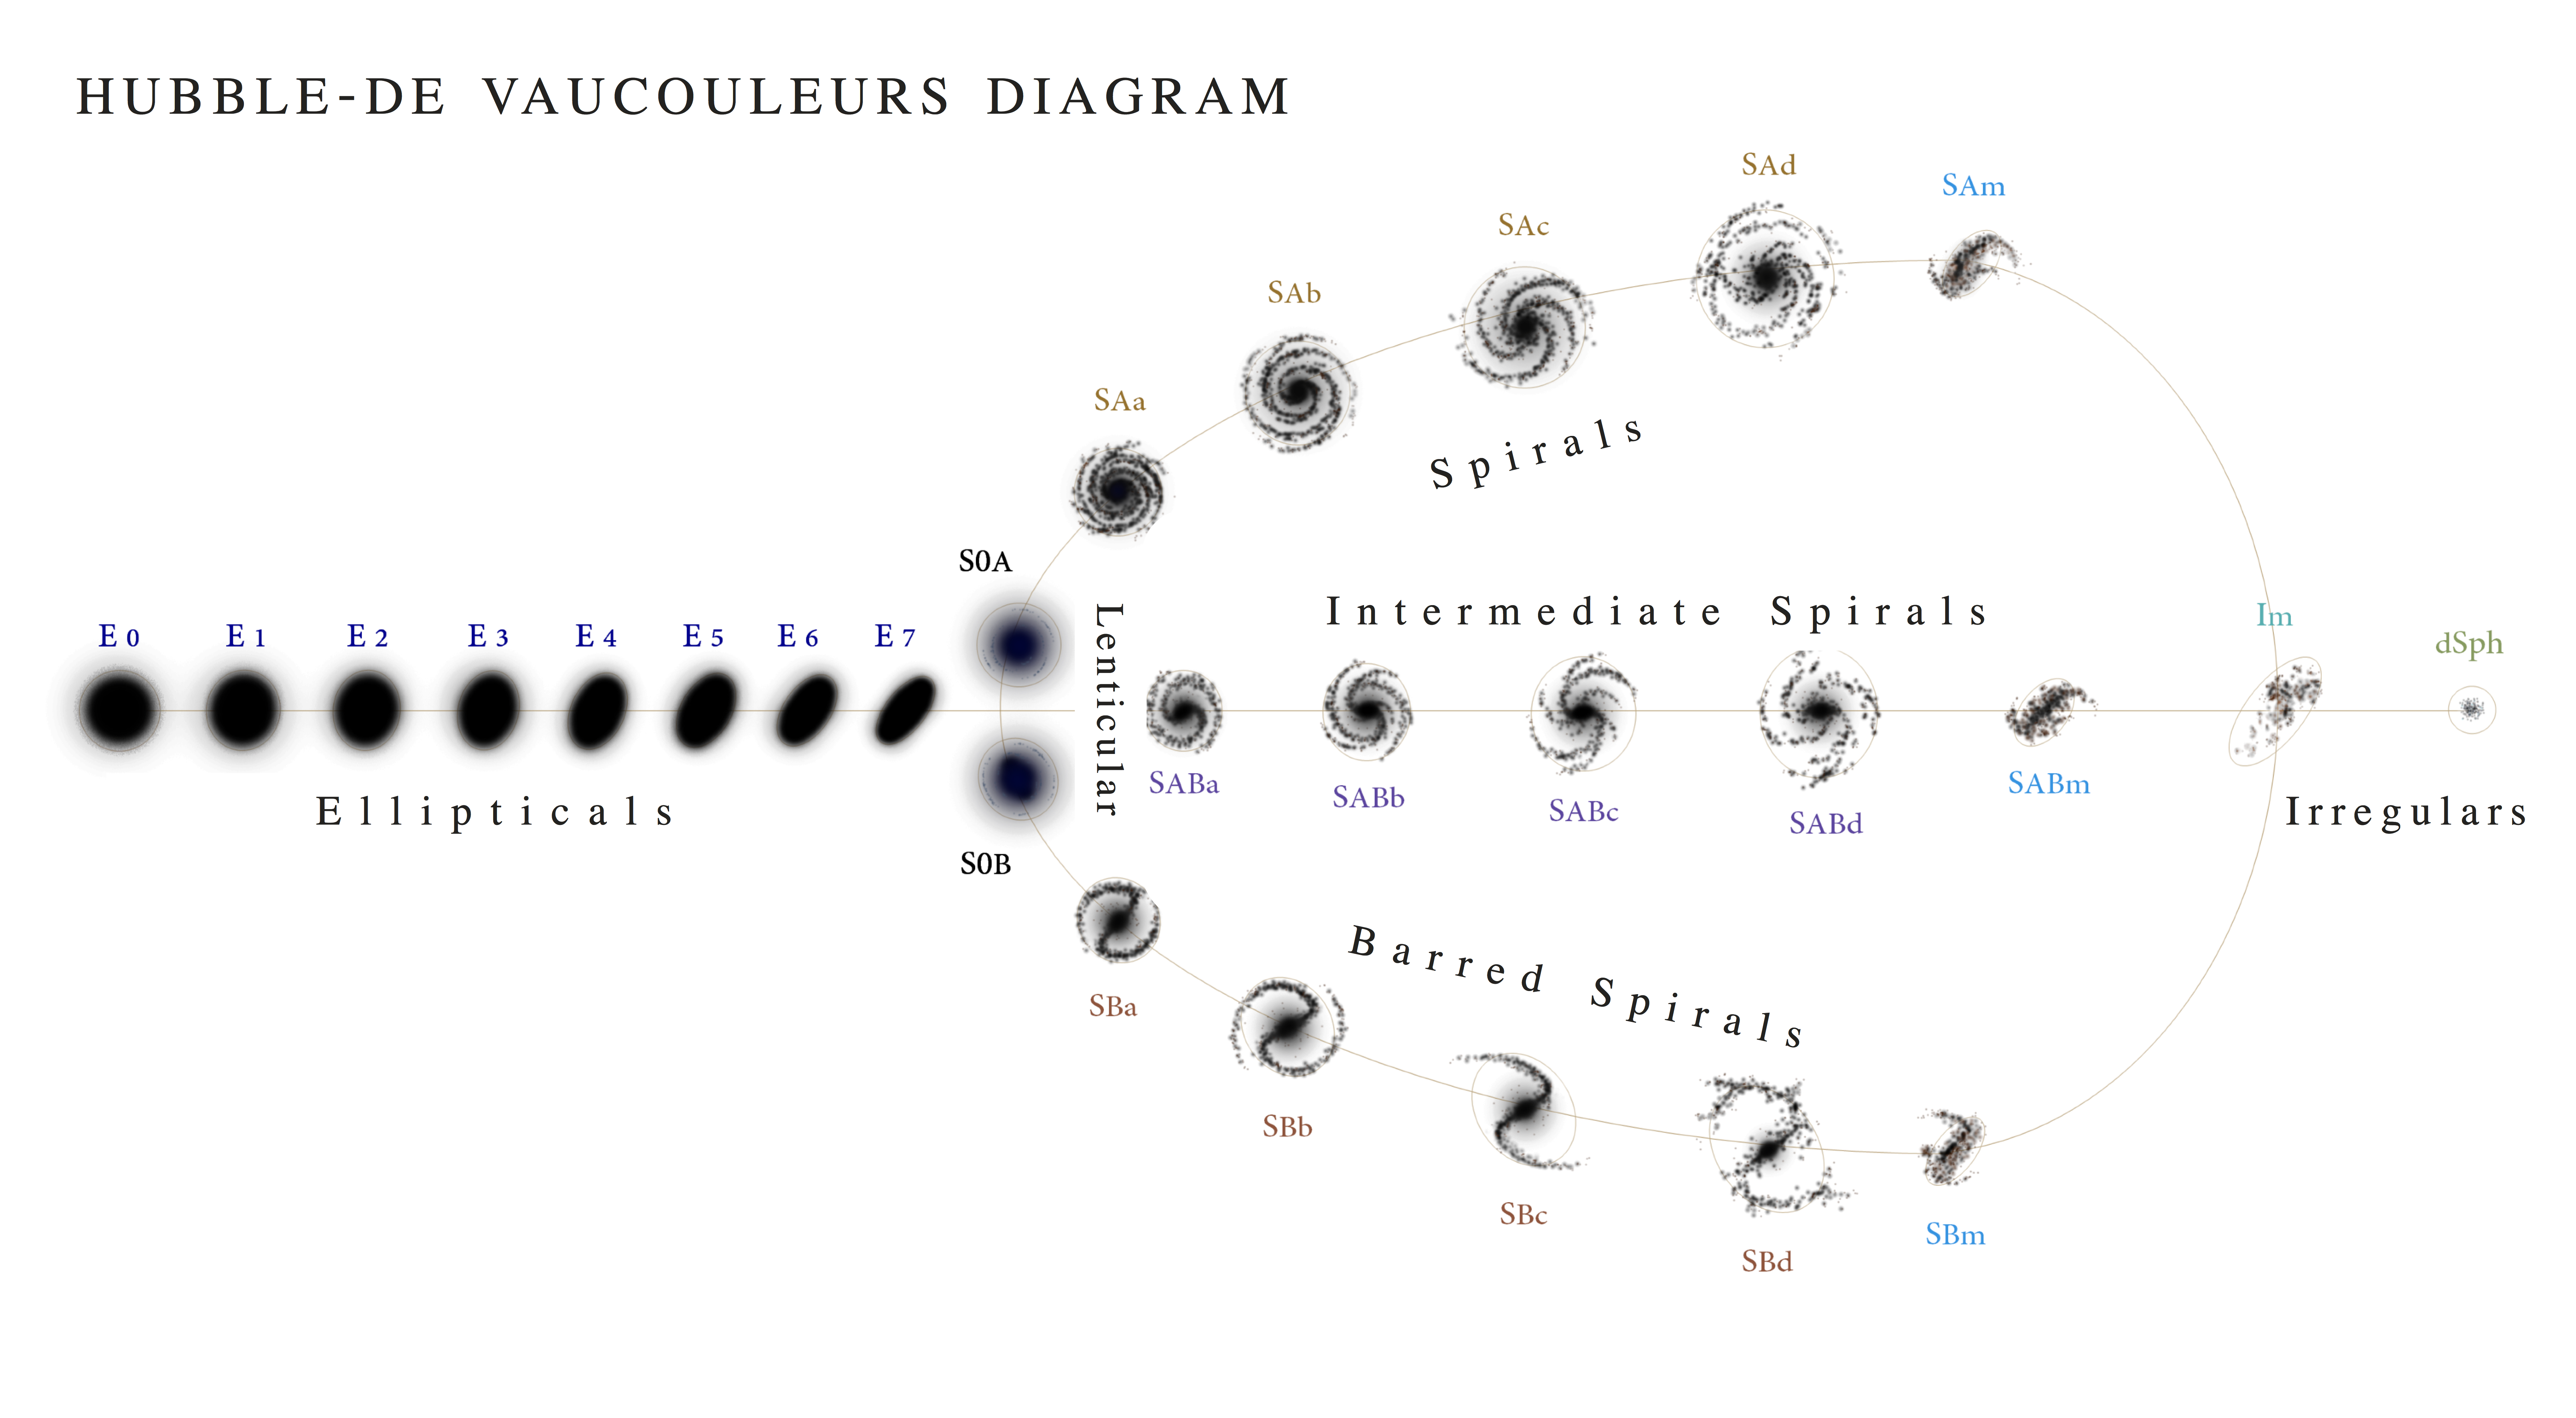
\includegraphics[width=\linewidth]{GalaxyClassificationChart}
	\caption{The Hubble-de Vaucouleurs diagram for galaxy morphology. It was originally proposed as a diagram for the evolution of galaxies over time but is now only used to show the different sub-classes of galaxy in the three main groups.}
	\label{fig:classDiagram}
\end{figure}

Since their discovery, many various types of galaxies have been identified and categorized into three main groups (Figure \ref{fig:classDiagram}):\footnote{https://commons.wikimedia.org/wiki/File:Hubble\_-\_de\_Vaucouleurs\_Galaxy\_Morphology\_Diagram.png} elliptical, spiral, and irregular.

\begin{figure}[H]
	\centering
	\begin{minipage}{0.48\textwidth}
		\centering
		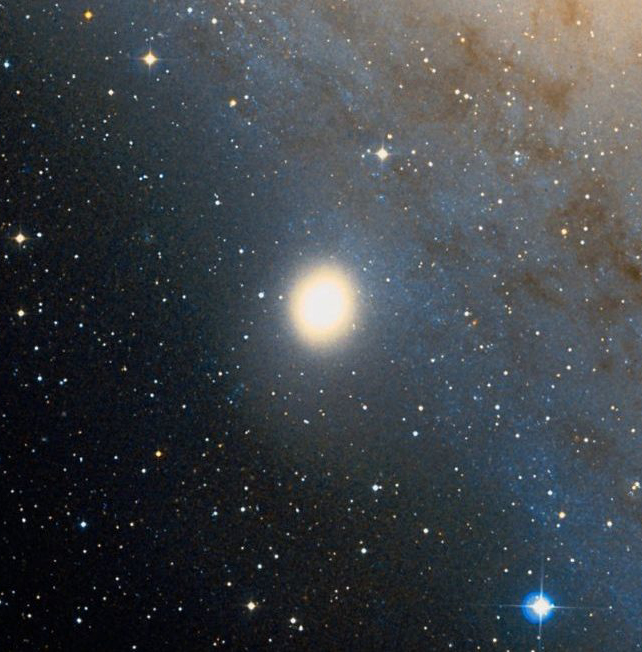
\includegraphics[width=0.9\linewidth]{M32}
		\caption{The elliptical galaxy M32 is gravitationally locked by the much larger galaxy Andromeda and is called a satellite galaxy as a result.}
		\label{fig:M32}
	\end{minipage}
	\begin{minipage}{0.04\textwidth}
		\centering
	\end{minipage}
	\begin{minipage}{0.48\textwidth}
		\centering
		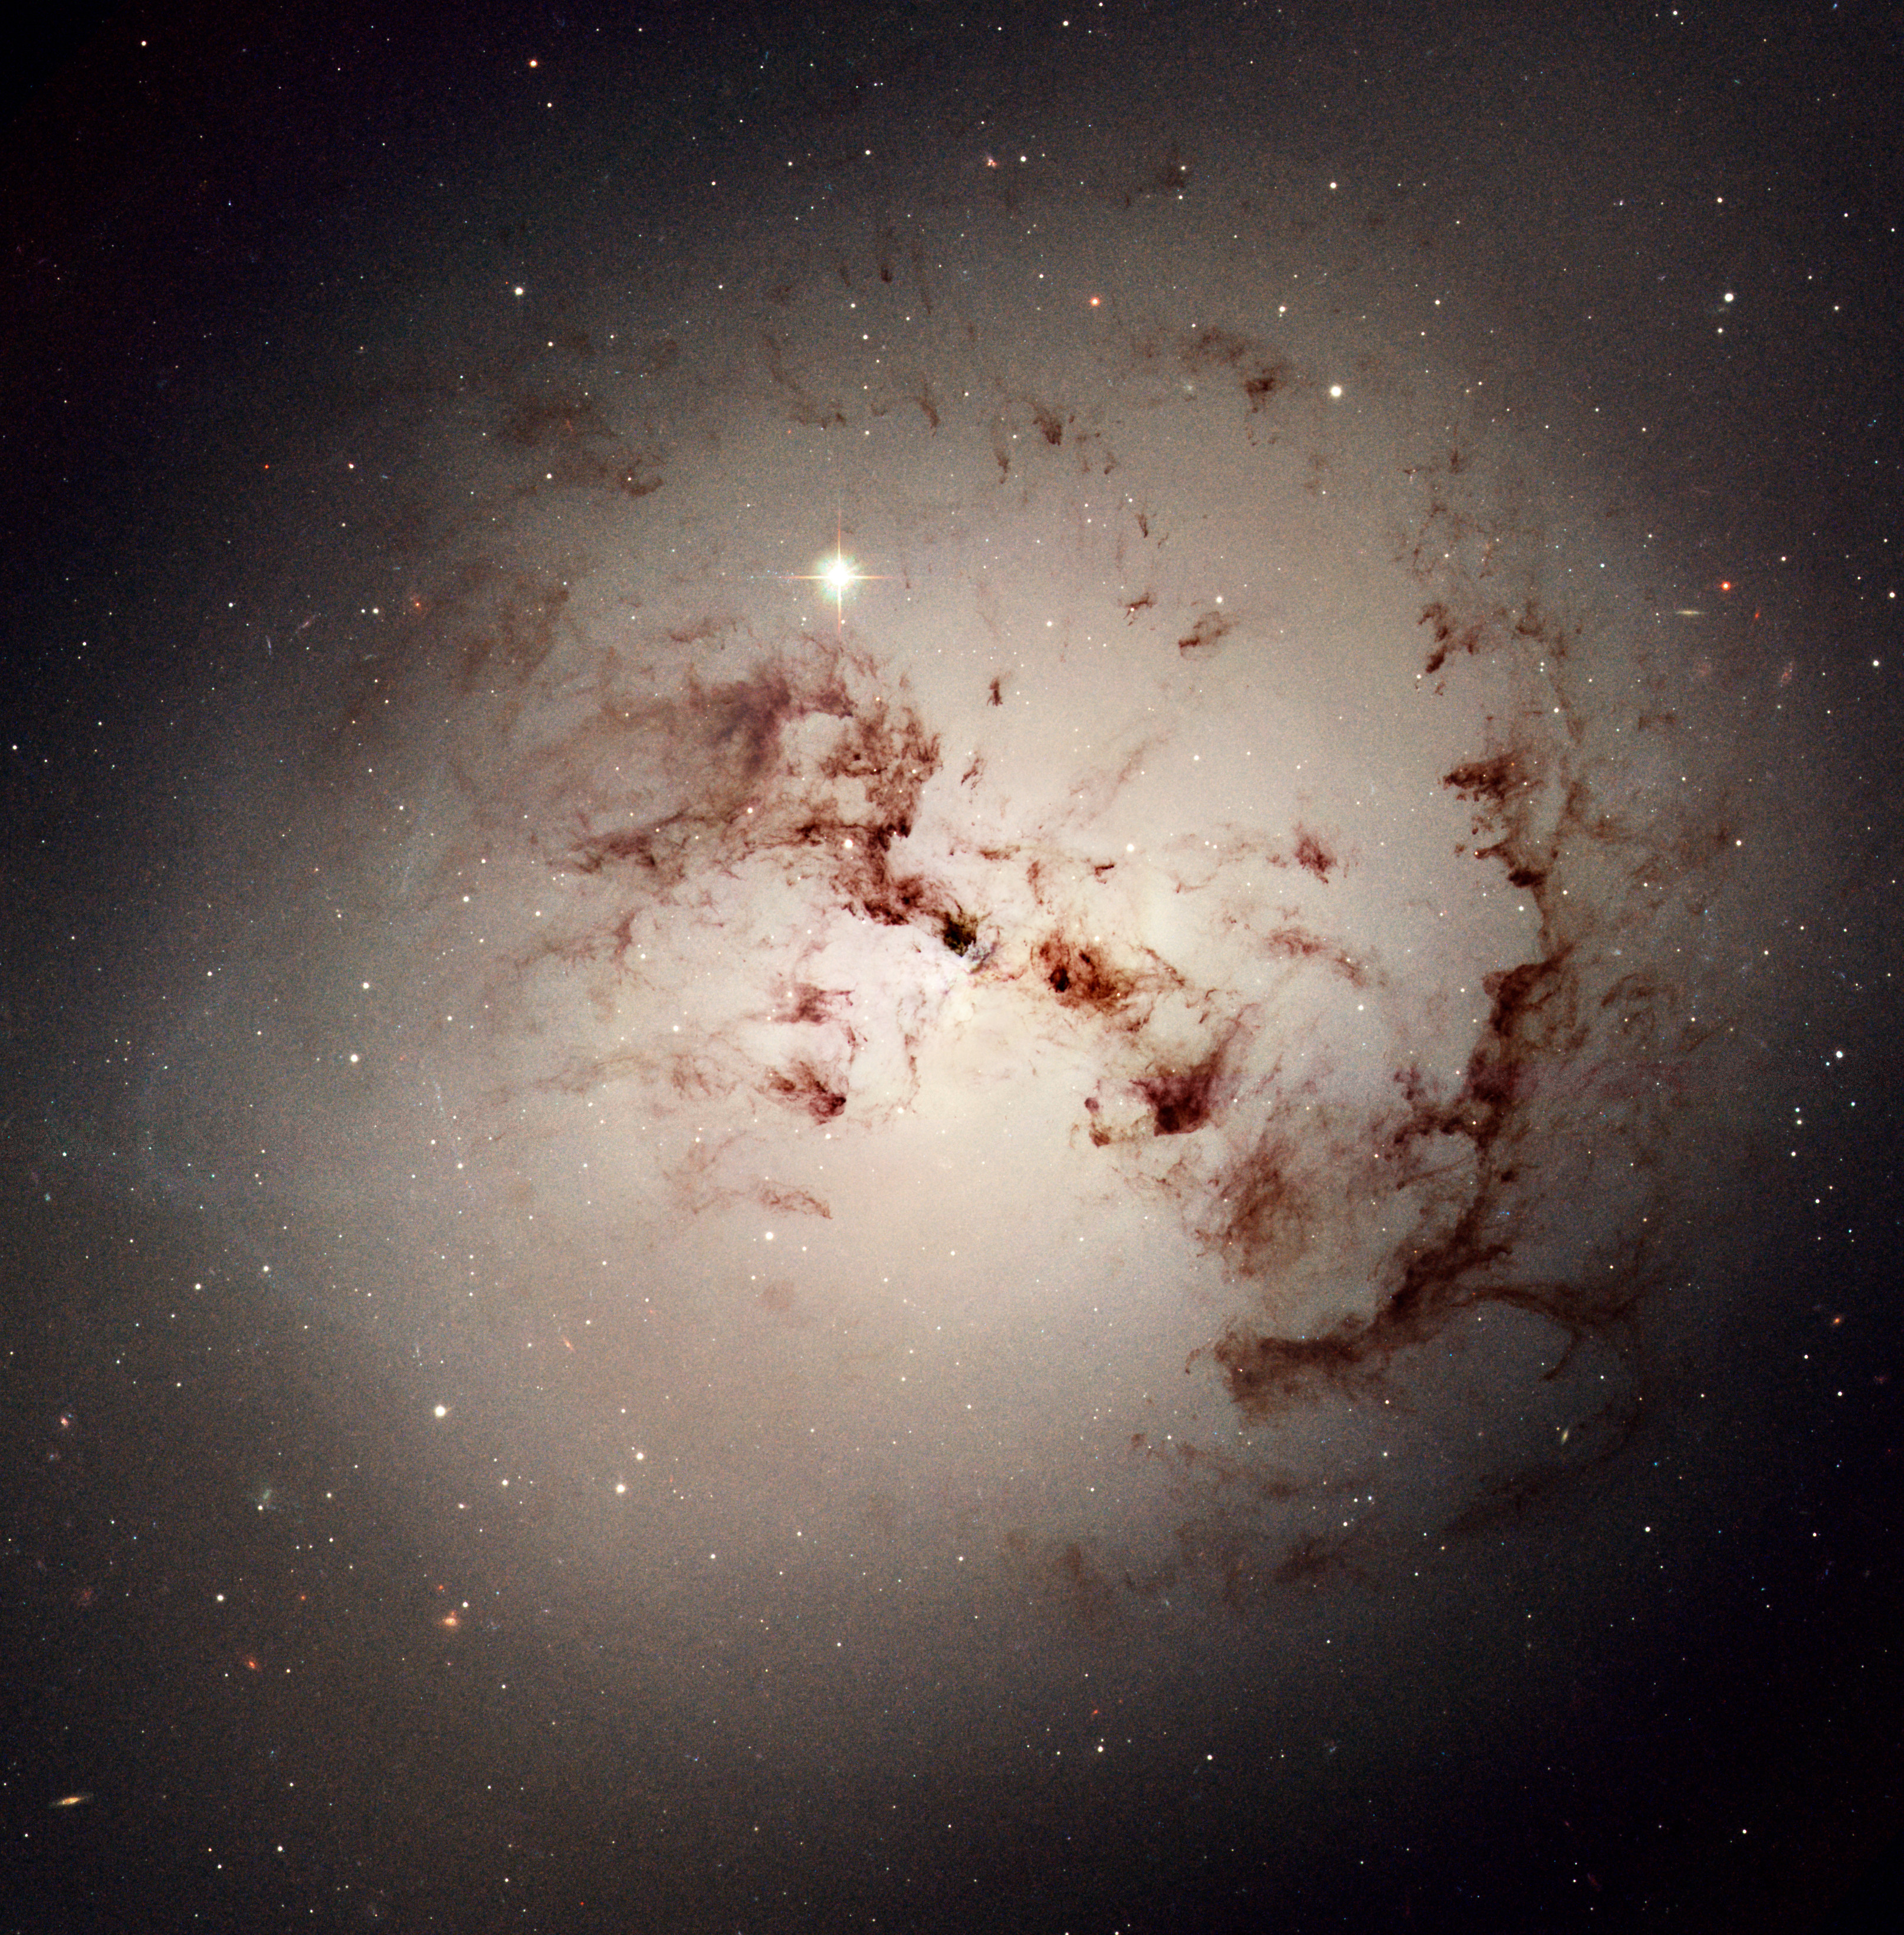
\includegraphics[width=0.9\linewidth]{NGC1316}
		\caption{The elliptical galaxy NGC 1316 has gas and dust lanes that make it look like a marble and are also evidence of a past merger.}
		\label{fig:NGC1316}
	\end{minipage}
\end{figure}

\subsection{\sc Elliptical Galaxies} \label{ellipticalGalaxies}

\cite{sag} describes elliptical galaxies as spherical or elliptical with no visible gas and dust and lacking young hot bright blue stars. These galaxies are classified from E0 to E7 based on how elliptical they appear from Earth and are the most abundant type of galaxy found in the observable universe. The dwarf satellite galaxy M32 is a nearby example of an elliptical galaxy (Figure \ref{fig:M32})\footnote{https://www.universetoday.com/wp-content/uploads/2009/07/Messier-32-e1484594524605.jpg}. The galaxy NGC 1316 (Figure \ref{fig:NGC1316})\footnote{ESA/Hubble \& NASA - https://www.spacetelescope.org/images/opo0511a/} is an unusual example of an elliptical galaxy in that it has lanes of gas and dust which is rare for ellipticals. The lanes of gas and dust that make it look like a marble are theorized to be the result of a merger of two galaxies at some time it its past.

\begin{figure}[H]
	\centering
	\begin{minipage}{0.48\textwidth}
		\centering
		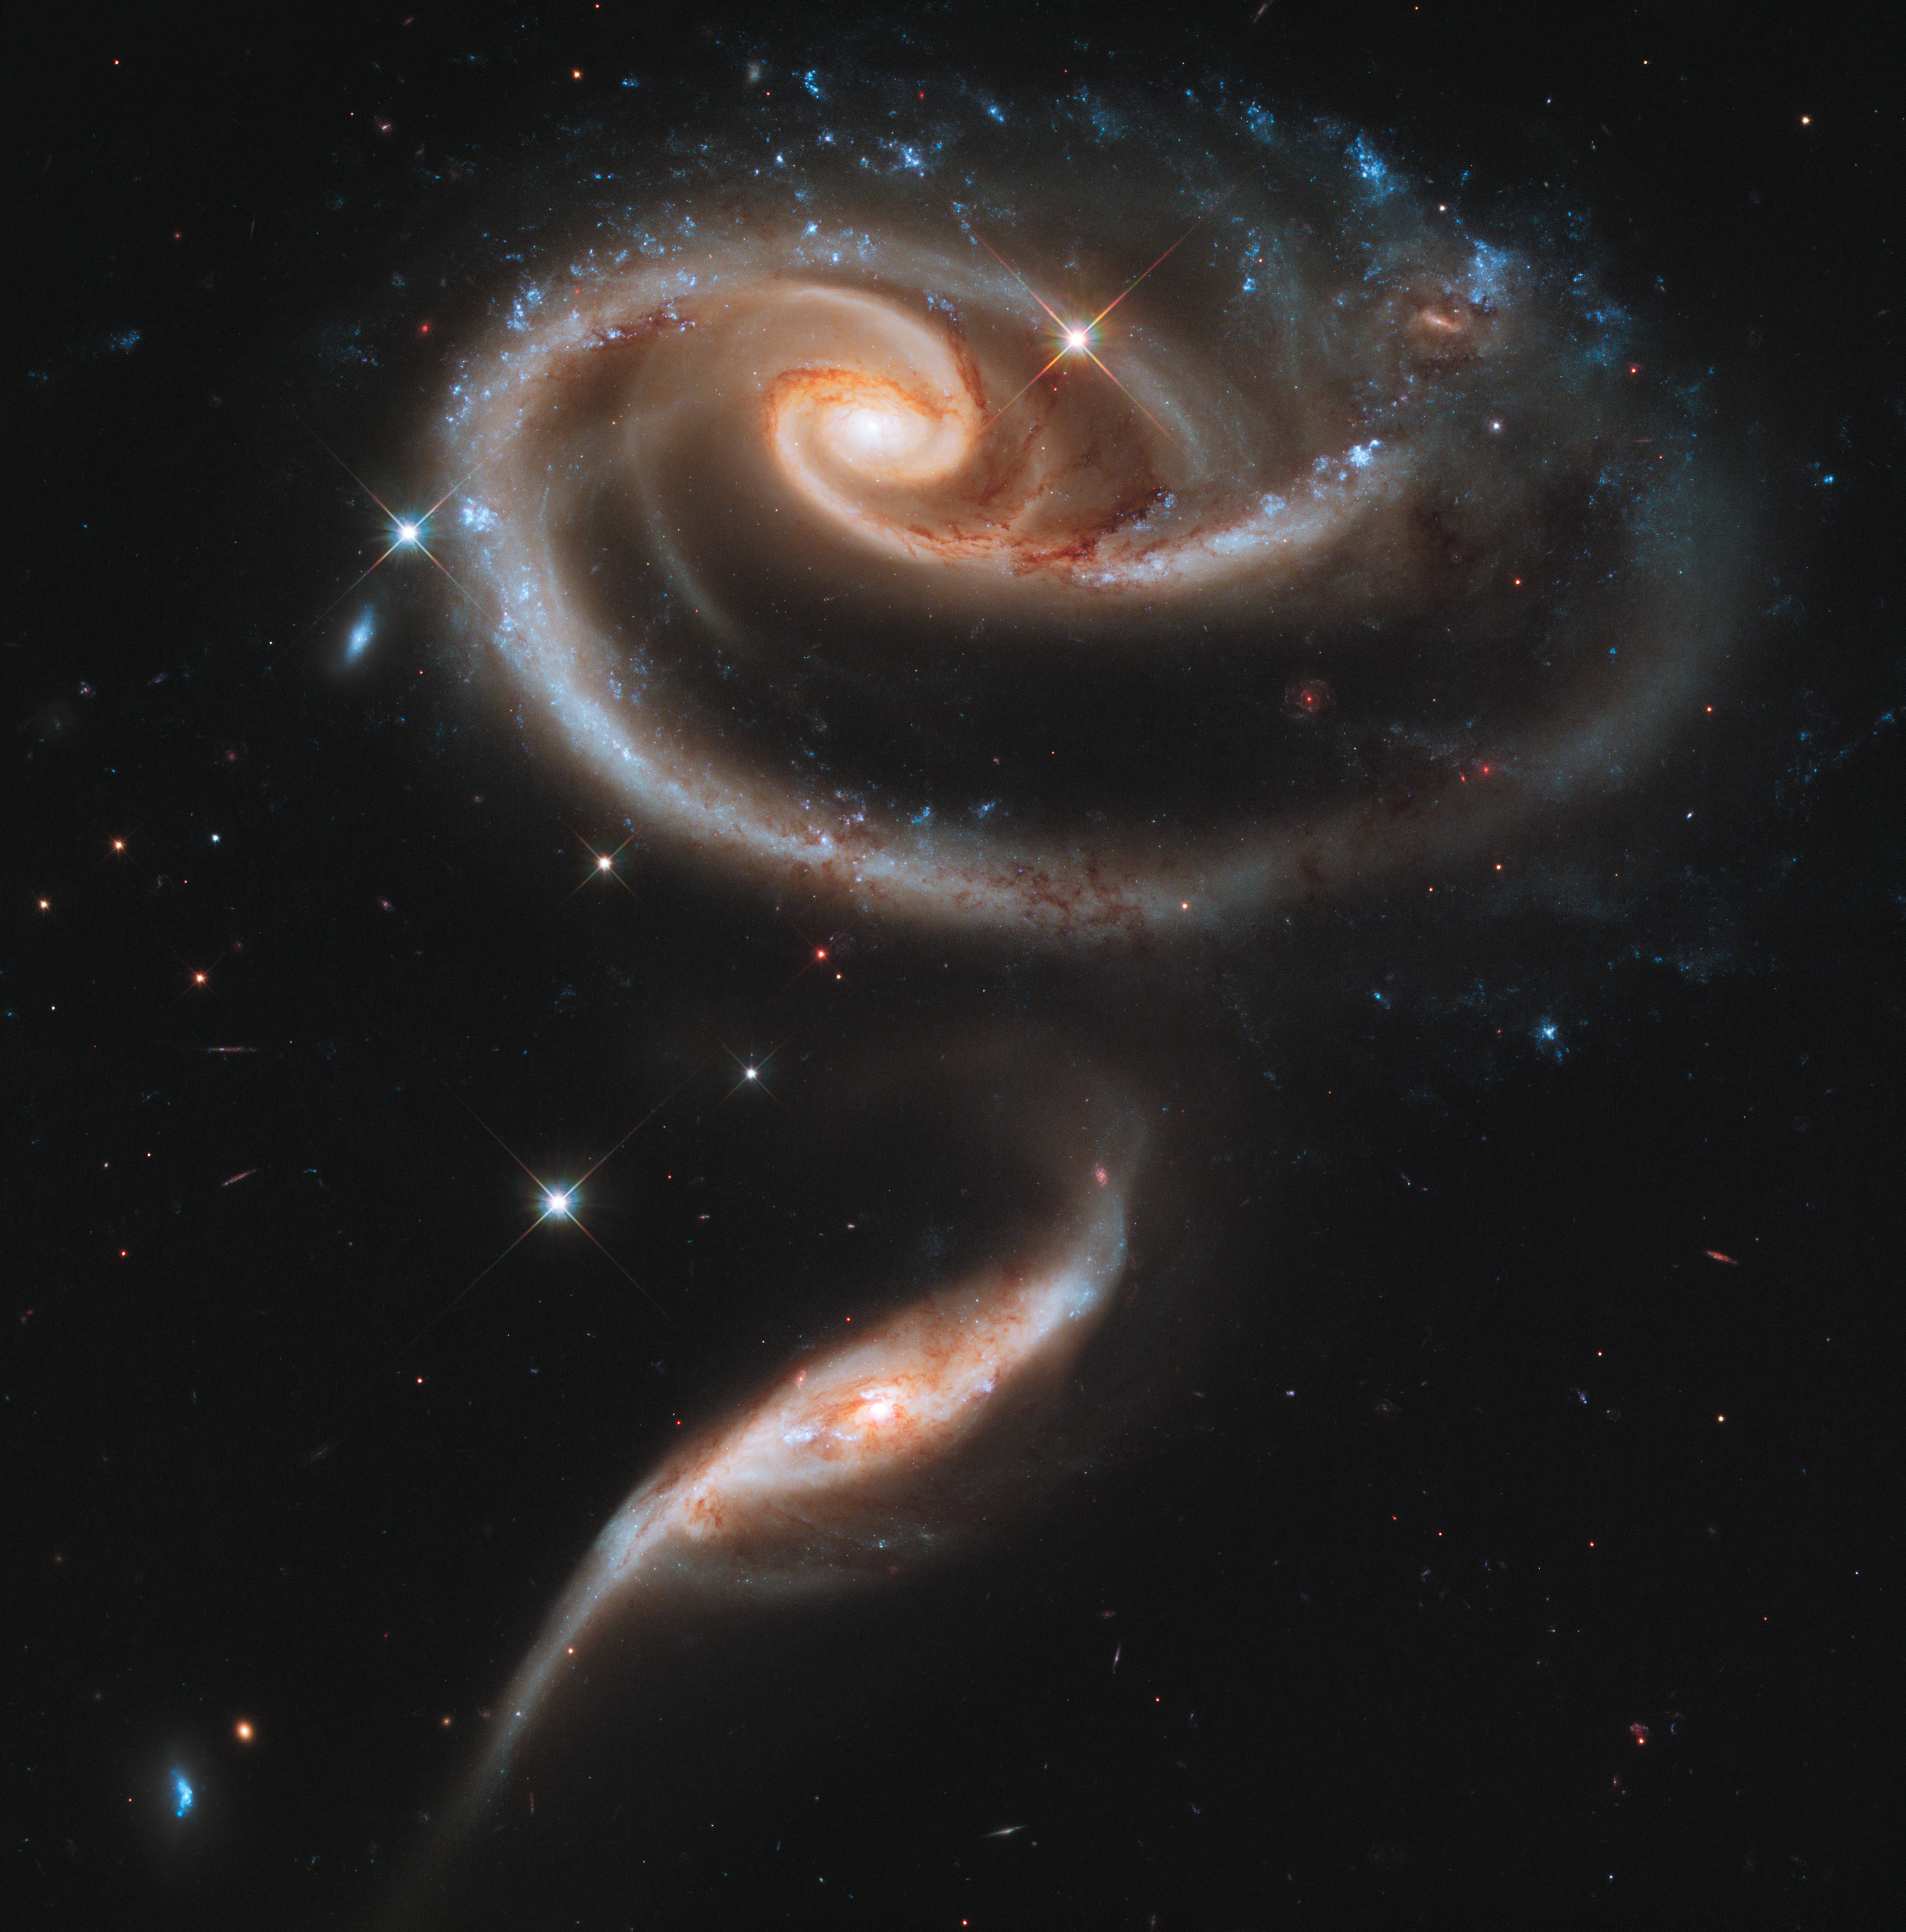
\includegraphics[width=0.9\linewidth]{Arp273}
		\caption{A pair of interacting galaxies known as Arp 273 hosts the spiral galaxy UGC 1810. It is thought that the smaller galaxy has passed through the larger one.}
		\label{fig:Arp273}
	\end{minipage}
	\begin{minipage}{0.04\textwidth}
		\centering
	\end{minipage}
	\begin{minipage}{0.48\textwidth}
		\centering
		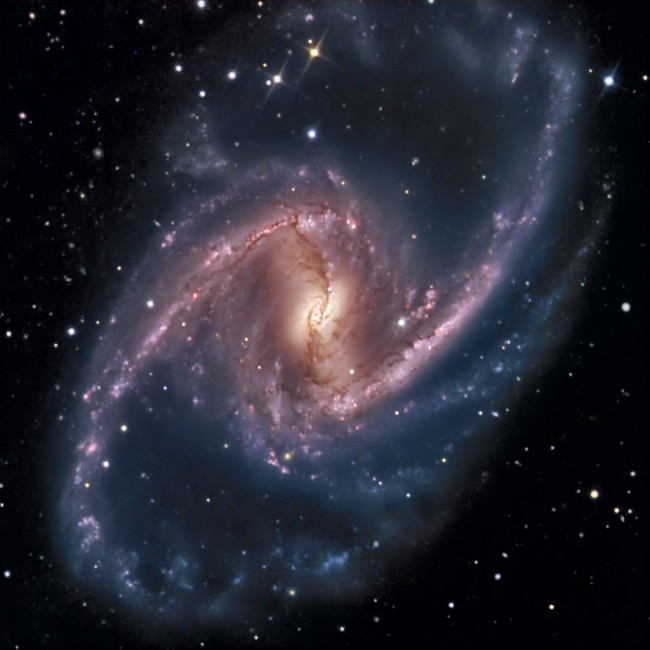
\includegraphics[width=0.9\linewidth]{NGC1365}
		\caption{The spiral galaxy NGC 1365 has an extremely prominent bar at its center that is thought to draw gas and dust into a star-forming maelstrom.}
		\label{fig:NGC1365}
	\end{minipage}
\end{figure}

\subsection{\sc Spiral Galaxies} \label{spiralGalaxies}

Spiral galaxies are photographically the most spectacular of the types (Figure \ref{fig:Arp273})\footnote{ESA/Hubble \& NASA - https://www.spacetelescope.org/images/heic1107a/} due to the spiraling arms that give them their name. They consist of a flattened disk, spiral arms extruding from their nucleus, typically contain lots of gas and dust, and are host to star-formation regions containing many young hot bright blue stars. The gas and dust in spiral galaxies tend to form clouds which become birthing grounds for these young hot stars. A sub-class of spiral galaxies known as barred spirals(Figure \ref{fig:NGC1365})\footnote{R.Gilbert,D.Goldman,J.Harvey,D.Verschatse - https://apod.nasa.gov/apod/ap070328.html} are so called because of the presence of a bar at their center from which their spiral arms protrude. Our own galaxy, The Milky Way, is one of these barred spirals.

\begin{figure}[H]
	\centering
	\begin{minipage}{0.48\textwidth}
		\centering
		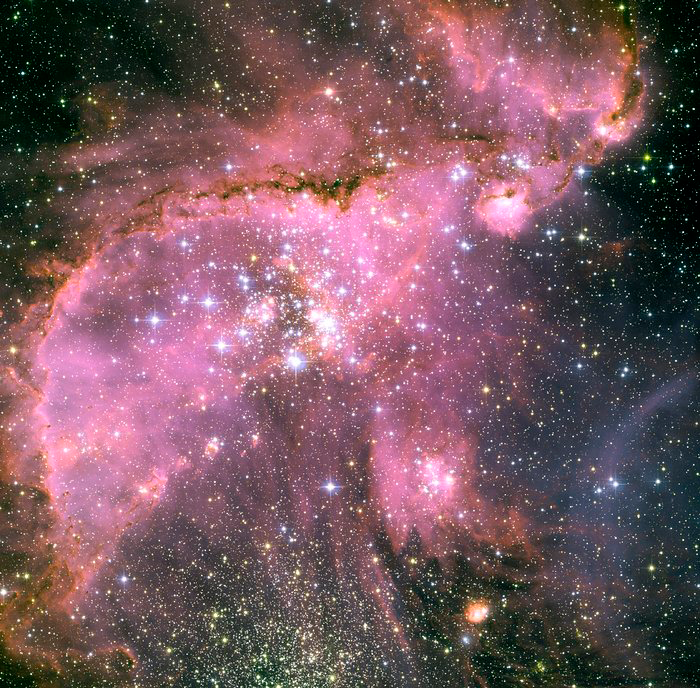
\includegraphics[width=0.9\linewidth]{SMC}
		\caption{The Small Magellanic Cloud has a spectacular looking dynamic and intricate star forming region.}
		\label{fig:SMC}
	\end{minipage}
	\begin{minipage}{0.04\textwidth}
		\centering
	\end{minipage}
	\begin{minipage}{0.48\textwidth}
		\centering
		\includegraphics[width=0.9\linewidth]{LMC}
		\caption{The Large Magellanic Cloud is host to one of the most active star formation regions in the nearby universe.}
		\label{fig:LMC}
	\end{minipage}
\end{figure}

\subsection{\sc Irregular Galaxies} \label{irregularGalaxies}

Not quite belonging to either the spiral nor the elliptical classes of galaxies, Irregular Galaxies are collections of gas and dust with no real structure or shape. Two examples of irregular galaxies close to our galaxy are the Magellanic Clouds. The Small Magellanic Cloud(Figure \ref{fig:SMC})\footnote{ESA/Hubble \& NASA - https://www.spacetelescope.org/images/heic0514a/} and Large Magellanic Cloud(Figure \ref{fig:LMC})\footnote{ESA/Hubble \& NASA - https://www.spacetelescope.org/images/heic1011a/} have virtually no proper geometric structure and are interacting gravitationally with the Milky Way galaxy.

\begin{figure}[H]
	\centering
	\begin{minipage}{0.48\textwidth}
		\centering
		\includegraphics[width=0.9\linewidth]{M82}
		\caption{The active galaxy M82 shown here in the visual range with hydrogen clouds shown in red.}
		\label{fig:M82}
	\end{minipage}
	\begin{minipage}{0.04\textwidth}
		\centering
	\end{minipage}
	\begin{minipage}{0.48\textwidth}
		\centering
		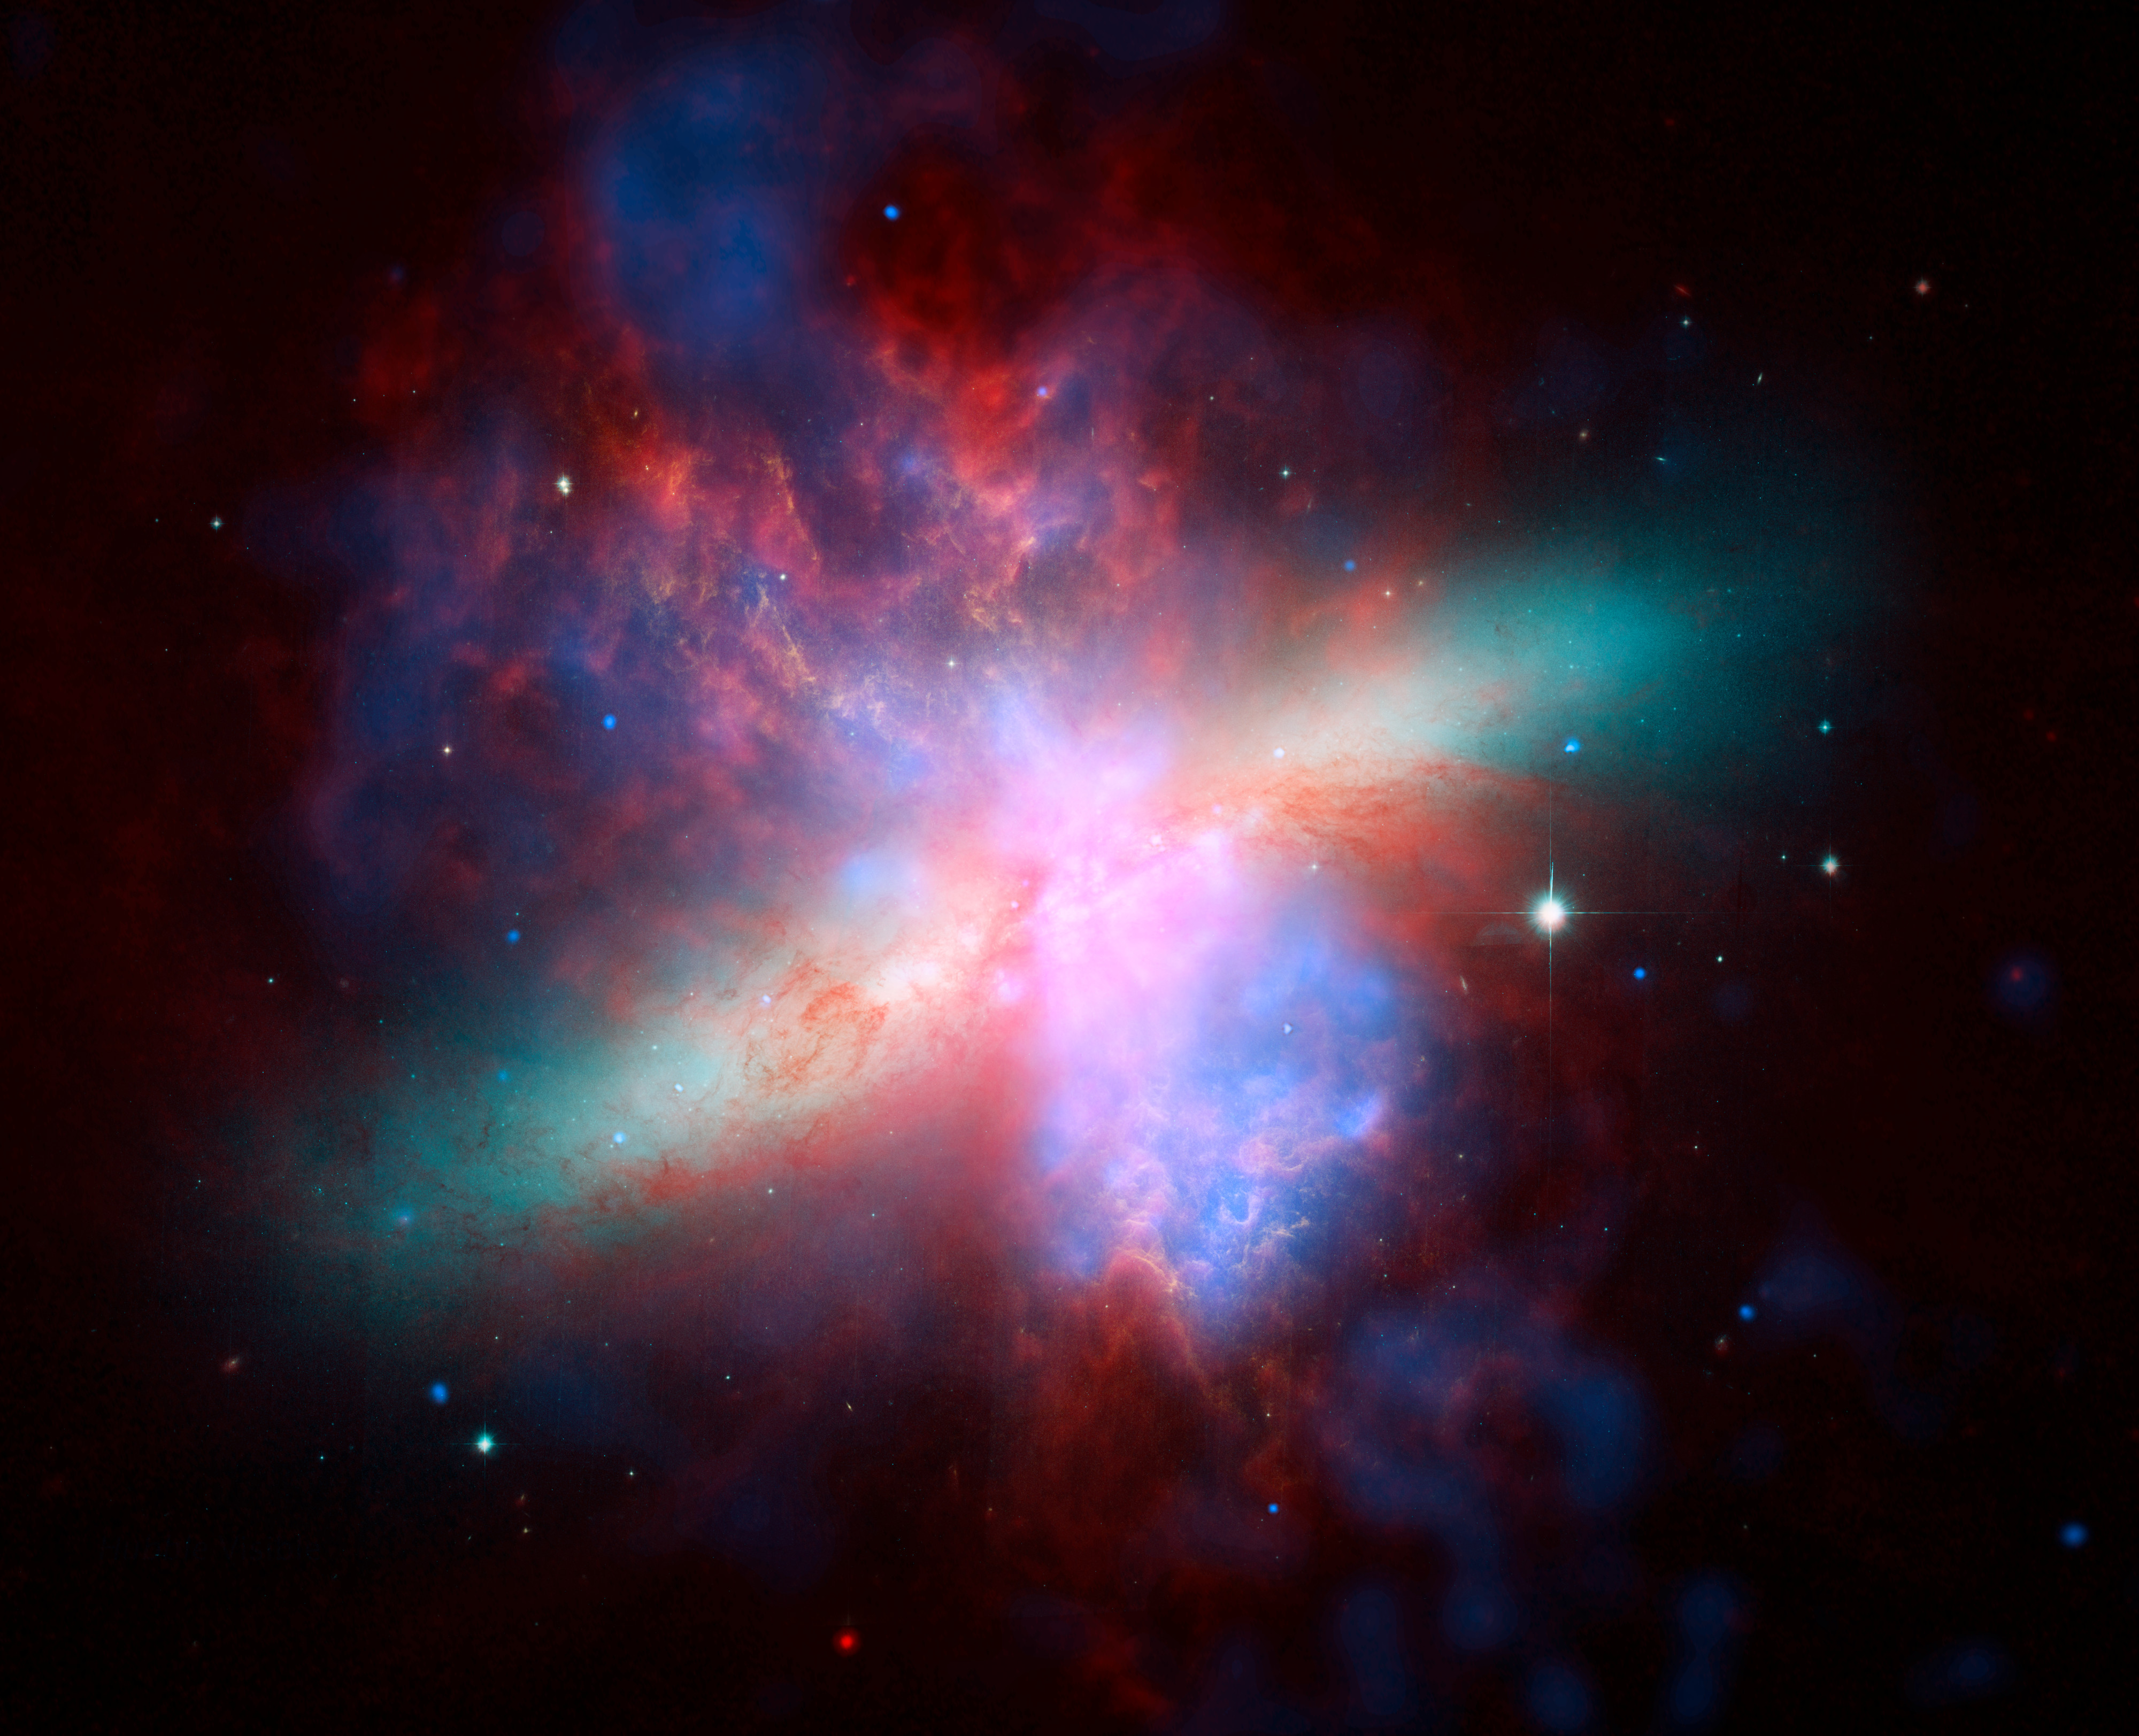
\includegraphics[width=0.87\linewidth]{M82-xray}
		\caption{The active galaxy M82 shown here with the radio loud hydrogen clouds in bright red and X-ray emission in blue.}
		\label{fig:M82-xray}
	\end{minipage}
\end{figure}

\section{\sc Active Galaxies} \label{activeGalaxies}

Thanks to advances in technology, such as the radio and X-ray telescopes, modern astronomers have identified a new type of galaxy. Active galaxies (Figure \ref{fig:M82})\footnote{ESA/Hubble \& NASA - https://www.spacetelescope.org/images/heic0604a/} are galaxies that are theorized to have an actively accreting supermassive black hole at their center. This accretion by the central black hole generates immense amounts of energy across the electromagnetic spectrum, particularly in the infrared and X-ray ranges of the EM spectrum (Figure \ref{fig:M82-xray})\footnote{ESA/Hubble \& NASA - https://www.spacetelescope.org/images/heic0604d/}. This central black hole and its accompanying accretion disc are known as the nucleus of an active galaxy and are referred to as Active Galactic Nuclei(AGN). There are a number of different types of AGN that have been identified based on their power spectra. Radio galaxies and their relatives the quasar and blazar are galaxies that are very luminous at radio wavelengths. The difference between radio galaxies, quasars, and blazars is that quasars and blazars are more luminous than radio galaxies with blazars being much more luminous than quasars. Radio galaxies, quasars, and blazars all emit jets from their centers and it is the angle of this jet with relation to us that causes the increase in radio emission in the quasars and blazars, see section \ref{unifiedModel}. Seyfert galaxies are like quasars in that they are very luminous in the radio wavelengths and are split into type I and type II based on their emission spectrum. What distinguishes Seyferts from quasars is that their host galaxies are clearly detectable.

\begin{figure}[H]
	\centering
	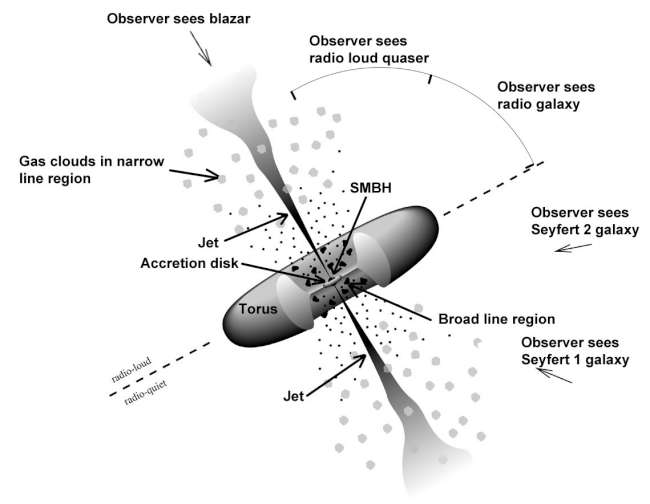
\includegraphics[width=0.6\linewidth]{UnifiedModel}
	\caption{Unified model of Active Galactic Nuclei (AGN).}
	\label{fig:unifiedModel}
\end{figure}

\subsection{\sc The Unified Model} \label{unifiedModel}

In order to help understand what we observe and to help produce new methods of observing AGN, the unified model was developed (Figure \ref{fig:unifiedModel}\footnote{https://fermi.gsfc.nasa.gov/science/eteu/agn/figure1.jpg}). 

In the unified model the nucleus of the active galaxy consists of a supermassive black hole surrounded by a torus of dust and gas from which it is accreting material from an accretion disc formed by the gravitational pull of the supermassive black hole. There are a number of different types of active galaxies that have been observed as discussed in section \ref{activeGalaxies}. The unified model attributes these different types to the viewing angle to the galaxy that the observer has. For instance if an observer is viewing an active galaxy from close to edge-on, then they will see either a radio galaxy or a Seyfert 2 AGN. If however they are observing from a higher angle, then the observer will see a quasar or a Seyfert 1 depending on whether the object is radio loud or not. Finally observing from an angle equivalent to directly above will result in the observer viewing a blazar.

\begin{figure}[H]
	\centering
	\begin{minipage}{0.6\linewidth}
		\centering
		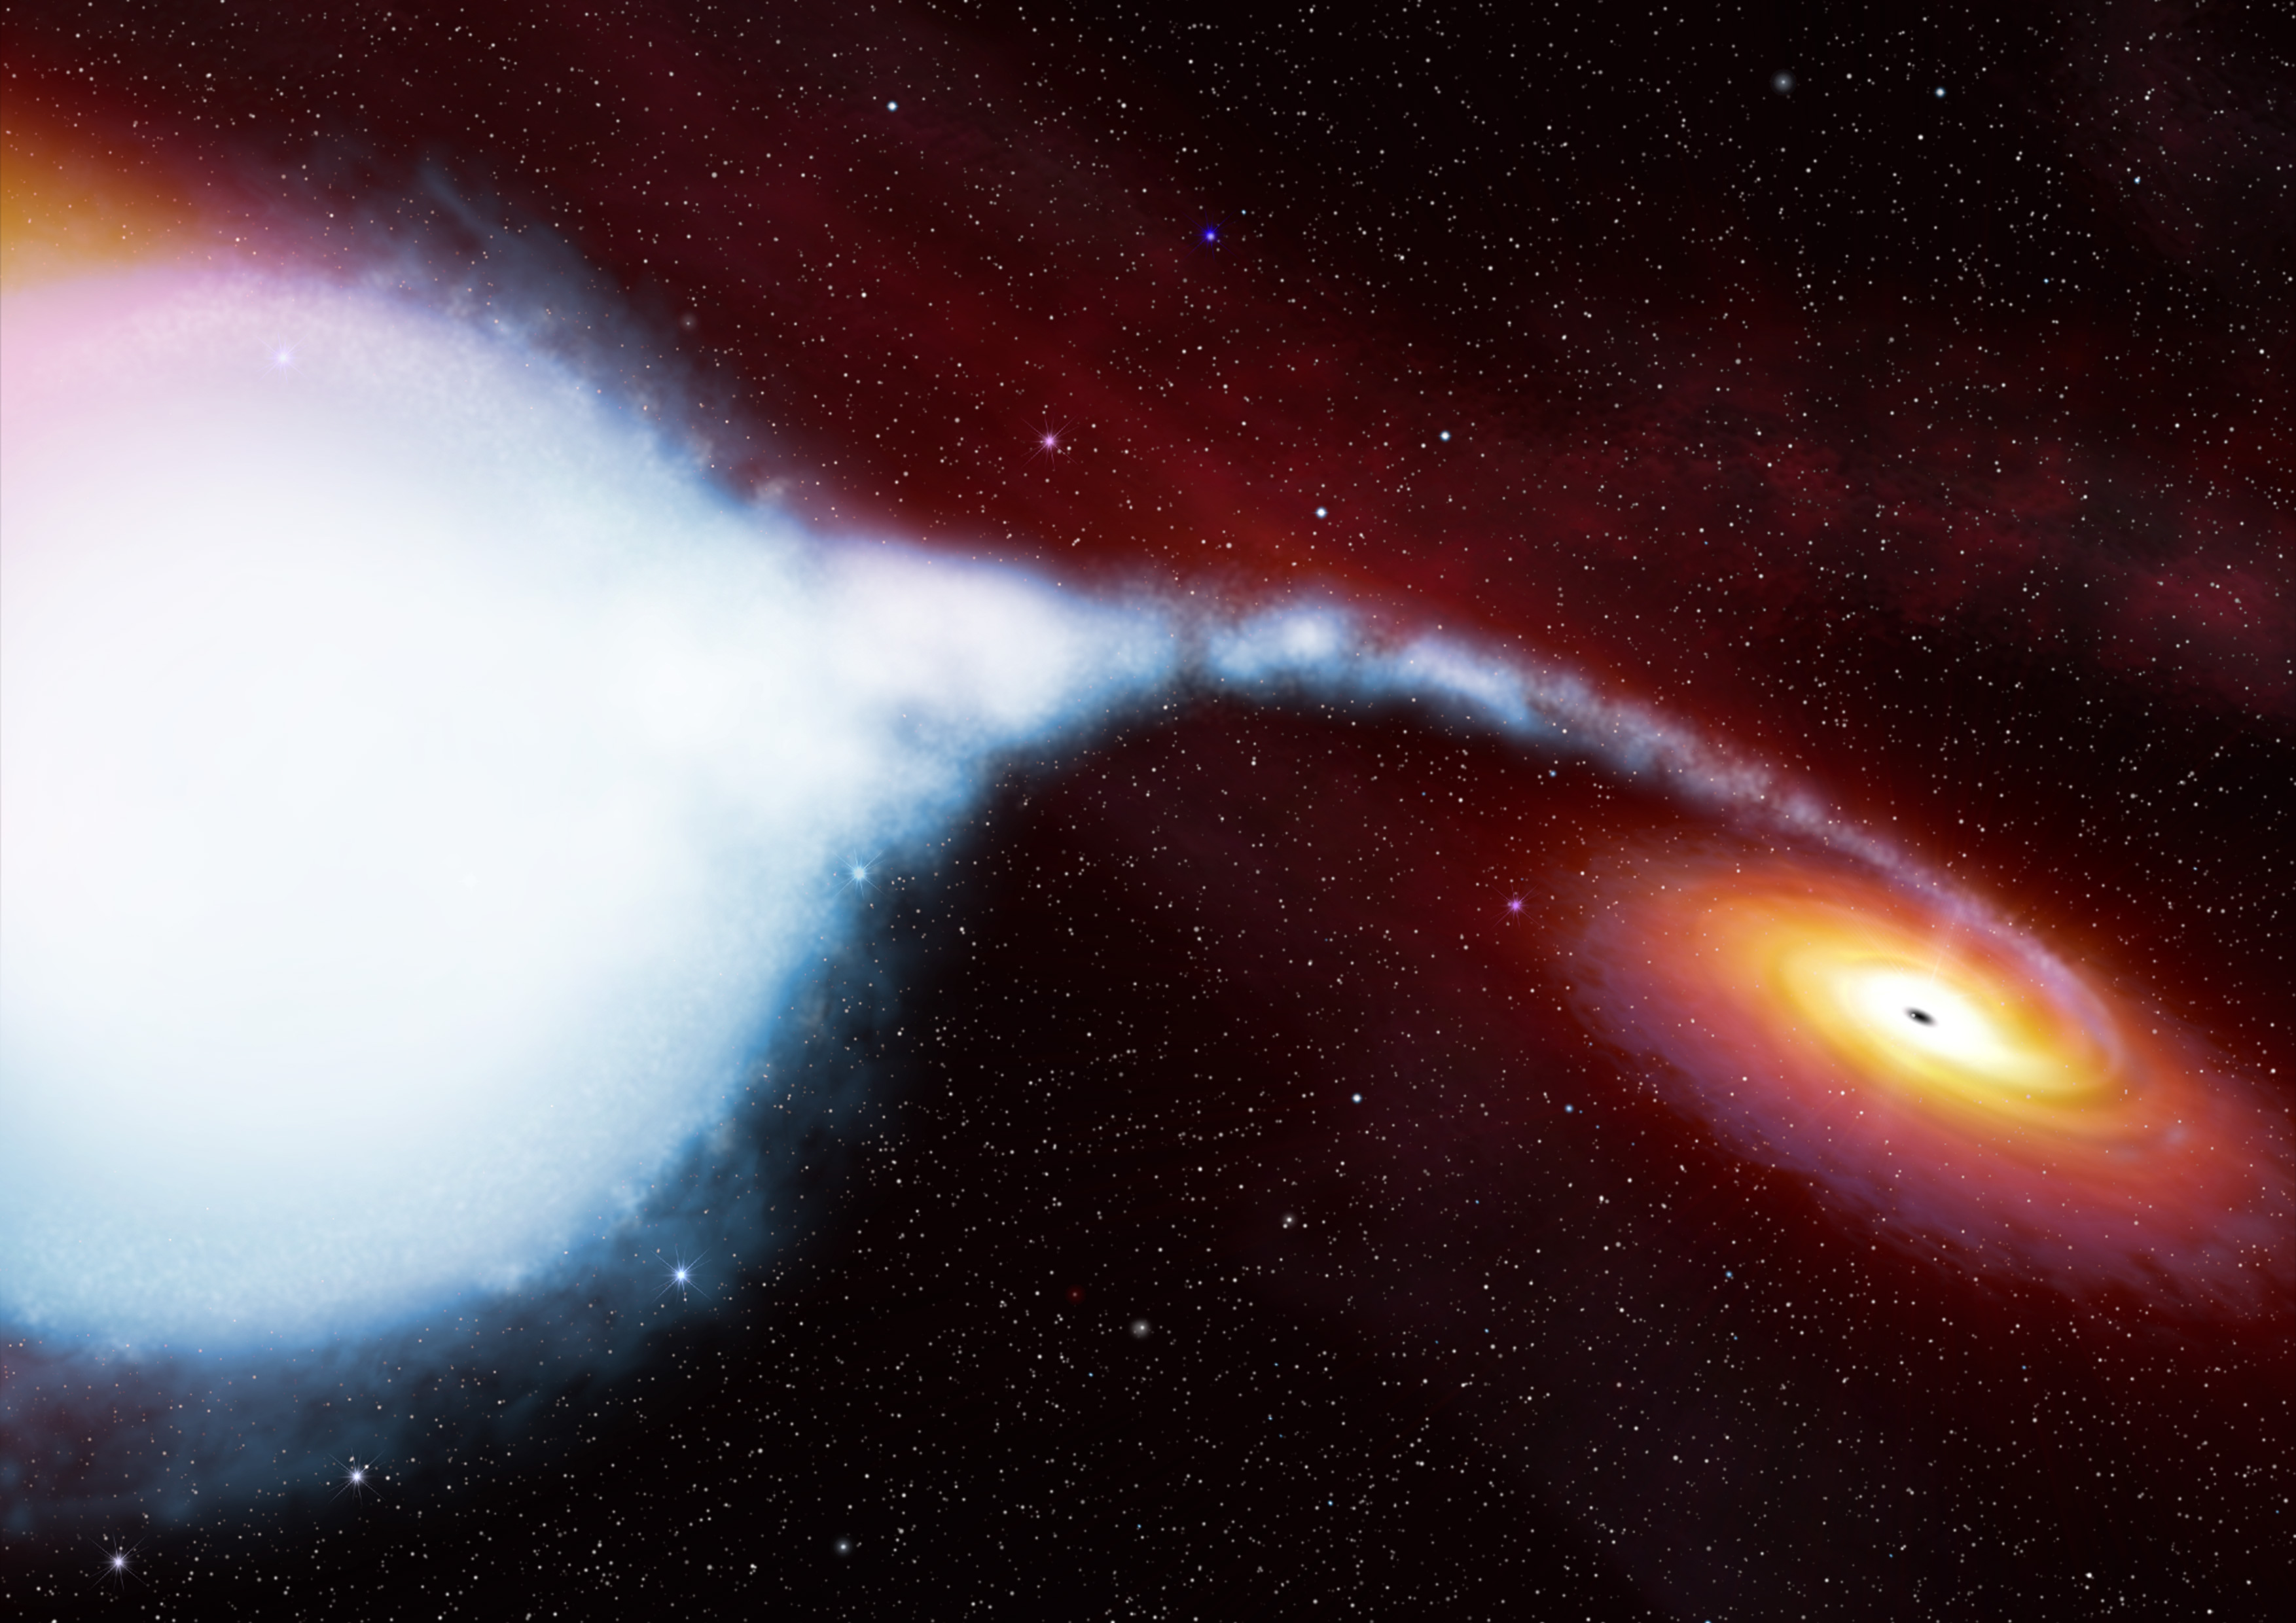
\includegraphics[width=0.8\linewidth]{CygX1}
		\caption{An artist's impression of the binary system to which Cygnus X-1 belongs.}
		\label{fig:CygX1}
	\end{minipage}
\end{figure}

\section{\sc Black Holes} \label{blackHole}

Black holes are stellar objects that emit no light themselves but have immense gravitational pulls. This often leads to the forming of accretion discs(Figure \ref{fig:CygX1})\footnote{ESA/Hubble \& NASA - https://www.spacetelescope.org/images/cygx1\_illust\_orig/} formed from the material of nearby objects. To understand black holes, one must first understand escape velocity and how it relates to astronomical objects. For any given object, the escape velocity is the velocity required by any object or particle in order for that object or particle to escape the gravitational well created by the initial object. For example, in order for a probe to leave our Earth and visit the other planets of our solar system, that probe must first reach the escape velocity for the Earth. Using Newtonian physics, the escape velocity is defined as:
\begin{equation} \label{eqn1.1}
v_{e} = \sqrt{\frac{2GM}{r}}
\end{equation}
where $v_{e}$ is the escape velocity, $G$ is the universal gravitational constant, $M$ is the mass of the object to escape from, and $r$ is the radius of the object. For an object of a given mass $M$, $v_{e}$ clearly increases as $r$ decreases. When $v_{e} \geq c$ at a given $r$, where $c \approx 3\cdot10^{8} \textup{m}/\textup{s}$ is the speed of light, then nothing can escape the gravitational well created by the object in question.

Such an object is referred to as a black hole. The radius at which the escape velocity reaches the speed of light, $v_{e} = c$, is called the event horizon. There exists a relativistic model for the black hole that will be discussed in chapter \ref{generalRelativity} that arises from general relativity. Black holes are commonly classified according to their mass due to the relationship between their mass and the radius of their event horizon, given by:
\begin{equation} \label{eqn1.2}
r_{s} = \frac{2GM}{c^{2}}
\end{equation}
where $r_{s}$ is known as the Schwarzchild radius and arises from setting the escape velocity $v_{e}$ equal to the speed of light in equation \ref{eqn1.1}.

\subsection{\sc Stellar Mass Black Holes} \label{stellarBH}

Stellar mass black holes are those black holes that have masses ranging from about $3\textup{M}_{\odot}$ to $10^{2}\textup{M}_{\odot}$ where $\textup{M}_{\odot}$ is the mass of our Sun. They are generally formed when the most massive stars die, ejecting their outer layers and collapsing in on themselves forming a black hole. Cygnus X-1 is an x-ray source from within the Milky Way that has widely been accepted to be a black hole, with a mass between 14 and 16 solar masses.

\subsection{\sc Intermediate-Mass Black Holes} \label{intermediateBH}

Intermediate-mass black holes(IMBH) are theorized to be those black holes with significantly more mass than a stellar mass black hole but less than a supermassive black hole. There are a few IMBH candidates in our own galaxy and in nearby galaxies. Intermediate-mass black holes have masses between $10^{2}\textup{M}_{\odot}$ and $10^{5}\textup{M}_{\odot}$ Since this thesis is concerned with AGN, and thus supermassive black holes, IMBHs will not be discussed further.

\subsection{\sc Supermassive Black Holes}

With masses ranging from $10^{5}\textup{M}_{\odot}$ and up, supermassive black holes are believed to be at the centers of most galaxies. There is observational evidence that our own Milky Way is host to one such supermassive black hole. It has been named Sagittarius A* and its latest estimated mass is $4.31\pm 0.38\cdot 10^{6}\textup{M}_{\odot}$ \cite{gillessen2009}. When one of these supermassive black holes is actively accreting from its surrounding galaxy, we describe it as the nucleus of an active galaxy as discussed in section \ref{activeGalaxies}. It is comforting to note that Sagittarius A*, the supermassive black hole at the center of The Milky Way, is quiescent, and thus not actively accreting, as the process of accretion generates immense amounts of x-ray and gamma ray emission.

\section{\sc How AGN are Observed} \label{howObserved}

AGN are so distant, and their central engines are so massive, that light cannot escape them. So how then can we observe them? The answer to that question is that we cannot and still have not \textit{directly} observed one yet. We can however indirectly observe them, by their gravitational effect on their surroundings, and in the case of AGN by observing the emission they produce through their accretion process.

As discussed earlier in section \ref{activeGalaxies}, the supermassive black holes at their centers are undergoing active accretion. This process causes matter to in-spiral towards the black hole at increasing speeds. The matter around the black hole rotates at an increasing rate as it approaches because it must conserve angular momentum. The gas and dust in the area around the nucleus of an AGN forms a torus, which then thins into a disc as it approaches the event horizon of the black hole. As matter from the torus gets closer to the event horizon and its velocity increases, it heats up to temperatures so that it eventually becomes ionized at the innermost stable circular orbit(ISCO).

The accretion disc matter becomes hot enough to emit light in the Ultra-Violet(UV) range, and electrons are striped and deposited into clouds above and below the disc. In these electron clouds, UV light rays collide with electrons and remove energy from them in a process known as Inverse Compton Scattering, commonly referred to as Inverse Comptonisation. The UV rays that undergo this Comptonising process are re-emitted at high energies, often in the X-ray band but also up to and including the gamma ray band.

\begin{figure}[H]
	\centering
	\begin{minipage}{0.8\linewidth}
		\centering
		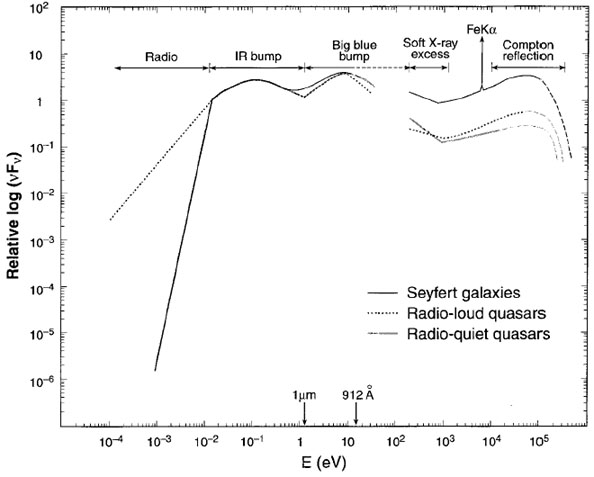
\includegraphics[width=0.8\linewidth]{AGN-spectra}
		\caption{Schematic representation of the broadband continuum spectral energy distribution seen in the different types of AGNs.}
		\label{fig:agn-continuum}
	\end{minipage}
\end{figure}

\subsection{\sc Light-Curves} \label{lightcurves}
Thanks to the processes in and around the accretion disc, AGN emit light almost evenly, with slight variations and perturbations, across the entire electromagnetic spectrum (Figure \ref{fig:agn-continuum})\footnote{https://ned.ipac.caltech.edu/level5/Sept04/Koratkar/Koratkar1.html} \cite{koratkar}. This allows us to collect the light they emit in our direction using telescopes and generate what are known as light-curves using computers. Light-curves are a comparison of flux to the wavelength, frequency, or energy level of light particles. When observing AGN it is common to refer to wavelengths of light by their corresponding energy levels in keV.

Some expected properties of the spectra obtained from AGN are, the presence of an iron line around the 6.5 keV mark, a falloff in photon counts as photon energy increases, and obscuring of the lower energy X-ray and higher energy UV range due to absorption in the torus and surrounding gas and dust around the central engine.

\subsection{\sc Orbital X-ray telescopes} \label{xrayTelesopes}

As discussed in the previous section \ref{lightcurves}, AGN produce light almost evenly across the electromagnetic spectrum. The section that astronomers studying AGN find the most interesting is the UV to X-ray region. Most EM radiation in the UV to gamma-ray region is completely absorbed in out atmosphere, therefore orbital satellite telescopes must be used to collect emissions from AGN. For this project the Neil Gehrels \textit{Swift} Observatory was used. The \textit{Swift} orbital telescope is equipped with a UV/Optical telescope, capable of obtaining spectra in the UV and optical ranges. \textit{Swift} is also equipped with an X-ray telescope for obtaining spectra in the X-ray band of the EM spectrum. 

\begin{figure}[H]
	\centering
	\begin{minipage}{0.45\textwidth}
		\centering
		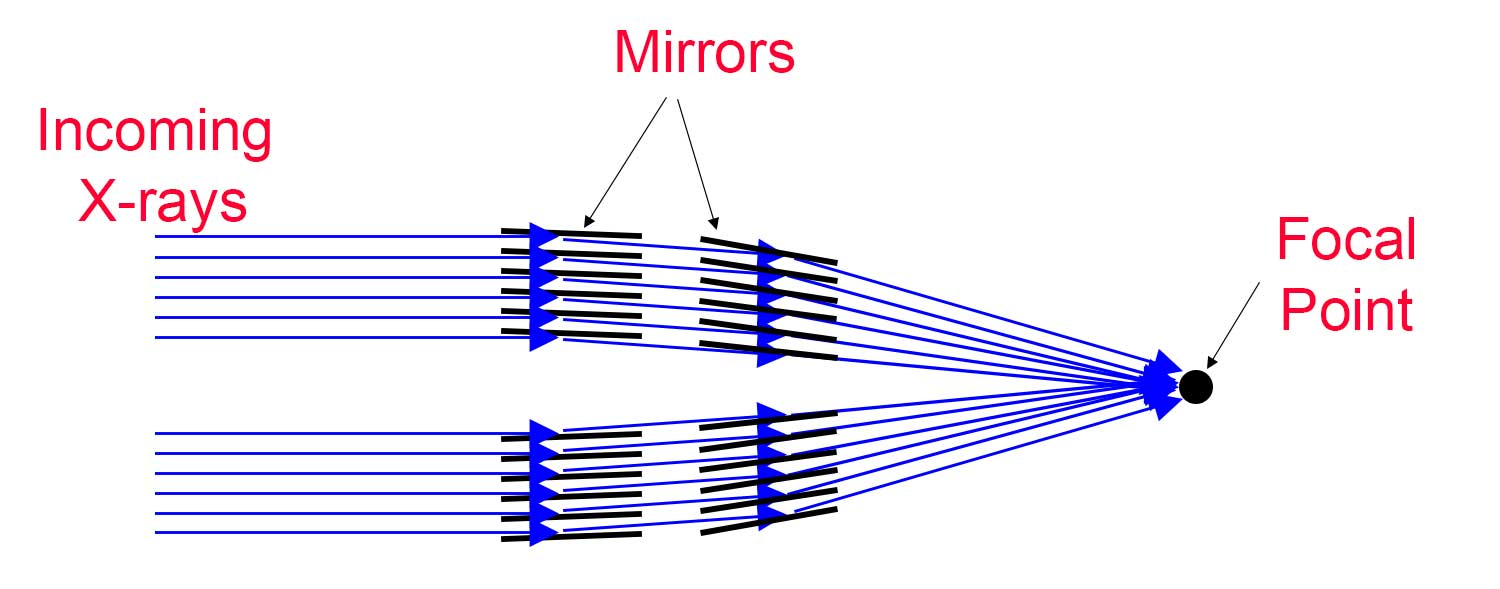
\includegraphics[width=\linewidth]{xrayTelescopeMultimirror}
		\caption{X-ray telescope cutaway diagram.}
		\label{fig:xrayMultiMirror}
	\end{minipage}
	\begin{minipage}{0.45\textwidth}
		\centering
		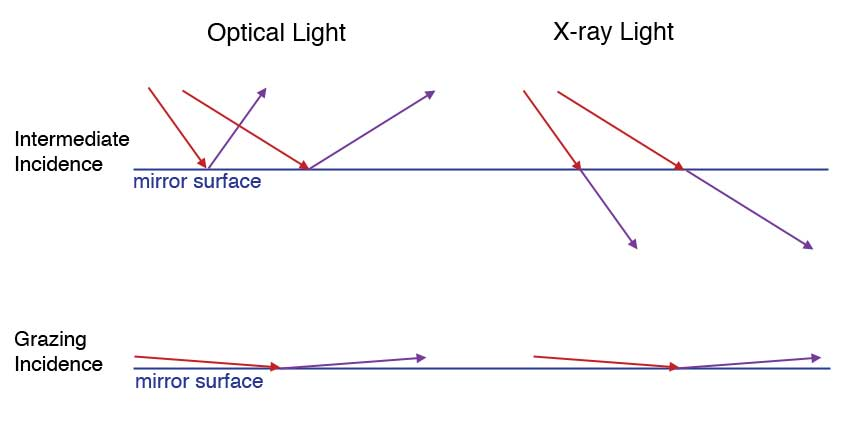
\includegraphics[width=\linewidth]{grazingIncidence}
		\caption{Grazing incidence diagram.}
		\label{fig:grazingIncidence}
	\end{minipage}
\end{figure}

The X-ray telescope uses many mirrors at slightly increasing angles positioned throughout to focus the incoming X-rays as shown in (Figure \ref{fig:xrayMultiMirror}\footnote{https://imagine.gsfc.nasa.gov/observatories/technology/xray\_telescopes1.html \label{xrayTelescopeRef}}). The mirrors must be placed at slightly increasing angles because otherwise, the high energy X-rays would pass right through the mirrors (Figure \ref{fig:grazingIncidence}\textsuperscript{\ref{xrayTelescopeRef}}).

\section{\sc Project Goals} \label{expectedAchievements}

This project focused on analyzing the light-curves of several AGN using a Structure Function. The Structure Function, as will be discussed in section \ref{structureFunction}, is similar to a Fourier Analysis but without the aliasing and windowing issues that arise from unevenly sampled data. We cannot obtain evenly sampled data from many astronomical sources due to the methods of observation and the timescales on which astronomical events happen. This project aims to provide a method for observing and analyzing astronomical events and objects such as AGN through the use of a Structure Function to help identify time-scales on which significant events might be occurring.

\chapter{\sc Relativistic Description of Black Holes} \label{generalRelativity}

Towards the end of the 17th century Newtonian gravity was still the accepted theory, however there still unexplained flaws in the theory that astronomers of the time struggled to explain. One of these such flaws was the behavior that Mercury exhibited in its orbit around the Sun. Mercury is a relatively small planet and as such it has lower mass than many of the other planets in the solar system. The combined mass of the planets further from the Sun than Mercury exhibit a gravitational pull on Mercury slowly altering its orbit (Figure \ref{fig:mercuryorbit})\footnote{https://www.ck12.org/physics/Orbital-Motion/rwa/Mercurys-Orbit/}. This precession could not be explained by the accepted model derived from Newtonian gravity. When Albert Einstein published his theory of General Relativity in 1915, it explained the precession of Mercury's orbit to the arcsecond.

General relativity, when observed from a stationary frame of reference, recovers Newtonian gravity. This is an extreme advantage because it means that in simple systems, Newtonian gravity can be used to perform predictions and calculations. When the gravitational force becomes great enough or the speed approaches the speed of light, Newtonian gravity starts to break down. It is in these instances that general relativity is required. The vicinity immediately surrounding black holes exerts gravitational forces so great that light is bent as a result, a phenomenon that cannot be explained within the constraints of Newtonian gravity.

Due to the masses of AGN and the requirement of General relativity to explain some of the processes inherent to them, this chapter will serve as a very brief overview of the mathematics of general relativity. AS it is a brief overview this chapter assumes that the reader has a sound mathematical background and is comfortable with concepts such as matrices, vectors, and partial differential equations.

\begin{figure}
	\centering
	\begin{minipage}{0.8\linewidth}
		\centering
		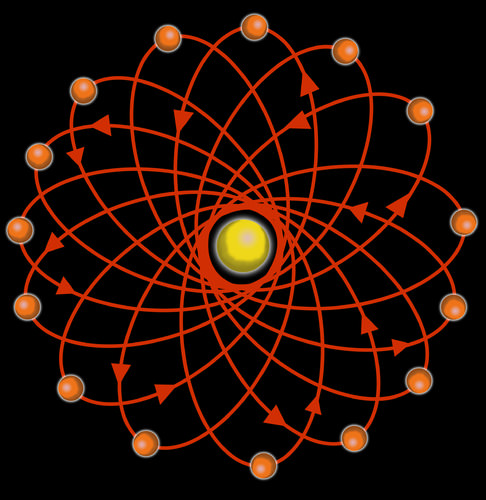
\includegraphics[width=0.8\linewidth]{mercury-orbit}
		\caption{Diagram depicting the precession of Mercury's orbit over time.}
		\label{fig:mercuryorbit}
	\end{minipage}
\end{figure}

\section{\sc An introduction to Tensors} \label{tensorIntro}

A fundamental and core building block of general relativity is the tensor. Tensors are mathematical objects that resemble matrices but obey a strict set of transformation laws. Tensors exist to help illustrate $m$-dimensional space. The rank, $n$, of a tensor is determined by the number of indices it has. For example the 3 dimensional vector $\xshlonghvecr{A}=0\hat{i} + 0 \hat{j} + 0 \hat{k}$ would be represented by a rank 1 tensor as $\contensor{A}{\alpha}$ where $\alpha = 1, 2, 3$. It is standard to reserve the $0^{th}$ dimension for the time dimension, and as such spacetime is represented by 4 dimensional tensors. A simple vector in spacetime would then be represented by $\contensor{A}{\alpha}$ where $\alpha=0,1,2,3$ and $\contensor{A}{0}$ would represent time. An important type of tensor is the one-form, which is equivalent to a scalar and has rank 0. 

As mentioned before, tensors can resemble matrices and as such matrices can be easily represented by a tensor. For example the matrix
\begin{equation}
\nonumber
A=
\begin{bmatrix}
1 & 2 & 3 \\
4 & 5 & 6 \\
7 & 8 & 9 \\
\end{bmatrix}
\end{equation}
would be represented by the tensor
\begin{equation}
\nonumber
\contensor{A}{ij}=
\begin{pmatrix}
1 & 2 & 3 \\
4 & 5 & 6 \\
7 & 8 & 9 \\
\end{pmatrix}
\end{equation}
while at first glance there doesn't seem to be any difference between the two, the tensor form has the advantage of being represented simply by $\contensor{A}{ij}$ where $i,j=1,2,3$.

In addition to tensors with upper indices, which are known as contravariant tensors, there are also tensors with lower indices defining covariant tensors. Mixed tensors are those tensors with both upper and lower indices. Any index that appears only once in a tensor equation is known is known as a free index whereas any index that is repeated can only be repeated once, and only as an upper and lower pair. This ties the repeated indices together as what is known as a dummy index and results in a sum over the paired dummy index. For example, given the two tensors $\contensor{a}{i}=\left(1, 2, 3\right)$ and $\covtensor{b}{i}=\left(4, 5, 6\right)$, their product $\contensor{a}{i}\covtensor{b}{i}$ is
\begin{eqnarray}
\nonumber
\contensor{a}{i}\covtensor{b}{i} &  = & \contensor{a}{1}\covtensor{b}{1} + \contensor{a}{2}\covtensor{b}{2} + \contensor{a}{3}\covtensor{b}{3}\\\nonumber
& = & (1)(4) + (2)(5) + (3)(6)\\\nonumber
& = & 4 + 10 + 18\\\nonumber
& = & 32
\end{eqnarray}

The final property of tensors that will be discussed is the general tensor transformation law. When transforming a tensor from one coordinate system, $\mixtensor{A}{ij}{kl}$, to another, $\mixtensor{A}{i'j'}{k'l'}$, tensors follow the general tensor transformation law
\begin{equation}
\mixtensor{A}{i'j'}{k'l'}=\frac{\partial x^{i'}}{\partial x^{i}}\frac{\partial x^{j'}}{\partial x^{j}}\cdot\cdot\cdot\frac{\partial x^{k}}{\partial x^{k'}}\frac{\partial x^{l}}{\partial x^{l'}}\cdot\cdot\cdot\mixtensor{A}{ij}{kl}
\end{equation} \label{eqn:tentran}
where the partial derivatives are the usual partial derivatives.

\section{\sc The Metric Tensor} \label{metricTensor}

There are some tensors in general relativity that are so important that they deserve naming. Of these named tensors, the metric Tensor is arguably the most important. The metric tensor, $\covtensor{g}{ij}$ or $\contensor{g}{ij}$, is used to express the unique distance between points in spacetime. The curvature of the spacetime has an effect on the metric tensor, for example in 3 dimensional flat spacetime is
\begin{equation}
\covtensor{g}{ij}=
\begin{pmatrix}
1 & 0 & 0 \\
0 & 1 & 0 \\
0 & 0 & 1 \\
\end{pmatrix}
\end{equation}\label{genten}
and when working with singularities such as black holes, the 4 dimensional metric tensor takes the form
\begin{equation}
\covtensor{g}{ij}=
\begin{pmatrix}
-1 & 0 & 0 & 0 \\
0 & 1 & 0 & 0 \\
0 & 0 & 1 & 0 \\
0 & 0 & 0 & 1 \\
\end{pmatrix}
\end{equation}\label{minkten}
and is named the Minkowski metric tensor after the mathematician Herman Minkowski \cite{spruin}. This particular form of the metric tensor takes its form as a result of the spacetime interval in 4 dimensional curved spacetime.

\section{\sc The Spacetime Interval} \label{spacetimeInterval}

In general relativity, we are often concerned with the infinitesimal distance between two points. This distance is conventionally denoted as $ds$ and it is trivial to see that in standard 3 dimensional space
\begin{equation}
\nonumber
ds^{2}=dx^{2}+dy^{2}+dz^{2}
\end{equation}
just as in two dimensional space $ds^{2}$ would be equivalent to Pythagorean. In 4 dimensional spacetime, the time dimension is subtracted, due to time only passing in one direction. This results in the spacetime interval
\begin{equation}
ds^{2}=-dt^{2}+dx^{2}+dy^{2}+dz^{2}
\end{equation}
and from here we can see why the Minkowski metric tensor(eqn \ref{minkten}) has a -1 at $\covtensor{g}{00}$ where the remaining diagonal terms are positive.

\section{\sc Black Hole Solutions} \label{blackHoleSolutions}

In astronomy black holes are frequently modeled using solutions to Einstein's field equations for general relativity.

\subsection{\sc The Schwarzchild Solution} \label{schwarzchildSolution}

The mathematics of the Schwarzchild solution.

\subsection{\sc The Kerr Solution} \label{kerrSolution}

The mathematics of the Kerr solution.

\subsection{\sc Properties of the Kerr Solution} \label{kerrSolutionProperties}

Properties of the Kerr solution.

%\chapter{\sc Statistical Analysis} \label{statisticalAnalysis}


\chapter{\sc The Structure Function} \label{structureFunction}

\section{\sc Mathematical Description} \label{mathematicalDesc}

Data collected on AGN is often difficult to work with, as mentioned in section \ref{activeGalaxies}, it is often unevenly sampled posing challenges to astronomers. Unevenly sampled data often causes aliasing and windowing when analyzed using conventional methods such as a Fourier-based power spectrum analysis. For this reason the method of structure function analysis was chosen, as it partially minimizes both aliasing and windowing. The structure function also has the added advantage of remaining in the time domain as opposed to the frequency domain as does the Fourier-based analysis. For these reasons the structure function was the method of choice for the analysis conducted in this project.

\subsection{\sc Definition of the Structure Function} \label{structureFunctionDefinition}

The structure function is discussed by \citep{cordes1985} in their appendix and was originally defined by \citep{rutman}. It can be closely compared to the auto-correlation and cross-correlation functions. Structure functions of order $M$ remove polynomials of order $M-1$ from the time series leaving a result that is dependent only on on any stationary random process inherent in the time series and any higher order polynomial trends.

For any given random process the $M^{th}$ order structure function is defined by \cite{rutman} as:
\begin{equation} \label{eqn3.1}
D^{\left(M\right)}_{\phi}\left(t, \tau\right) = \langle\left[\Delta^{\left(M\right)}_{\phi}\left(t, \tau\right)\right]^{2}\rangle
\end{equation}
where the angled brackets are an average over time $t$. \cite{rutman} also defines the $M^{th}$ increment of $\phi\left(t\right)$ as:
\begin{equation} \label{eqn3.2}
\Delta^{\left(M\right)}_{\phi}\left(t, \tau\right) = \sum_{n=0}^{\infty}\left(-1\right)^{n}{M \choose n}\phi\left(t + \left[M - n\right]\tau\right)
\end{equation}

For a time series of measurements $f\left(t_{i}\right), i = 1,2,3,...$ the first order structure is defined by \citep{collier2001} as:
\begin{equation}
S\left(\tau\right) = \frac{1}{N\left(\tau\right)}\sum_{i<j}\left[f\left(t_{i}\right)-f\left(t_{j}\right)\right]^{2}
\end{equation}
where the sum is over all pairs $\left(f\left(t_{i}\right),f\left(t_{j}\right)\right)$ for which $t_{j}-t_{i}=\tau$, and $N\left(\tau\right)$ is the number of such pairs.

\subsection{\sc Shape and Characteristics} \label{shapeAndCharacteristics}

\begin{figure}
	\centering
	\begin{minipage}{0.45\textwidth}
		\centering
		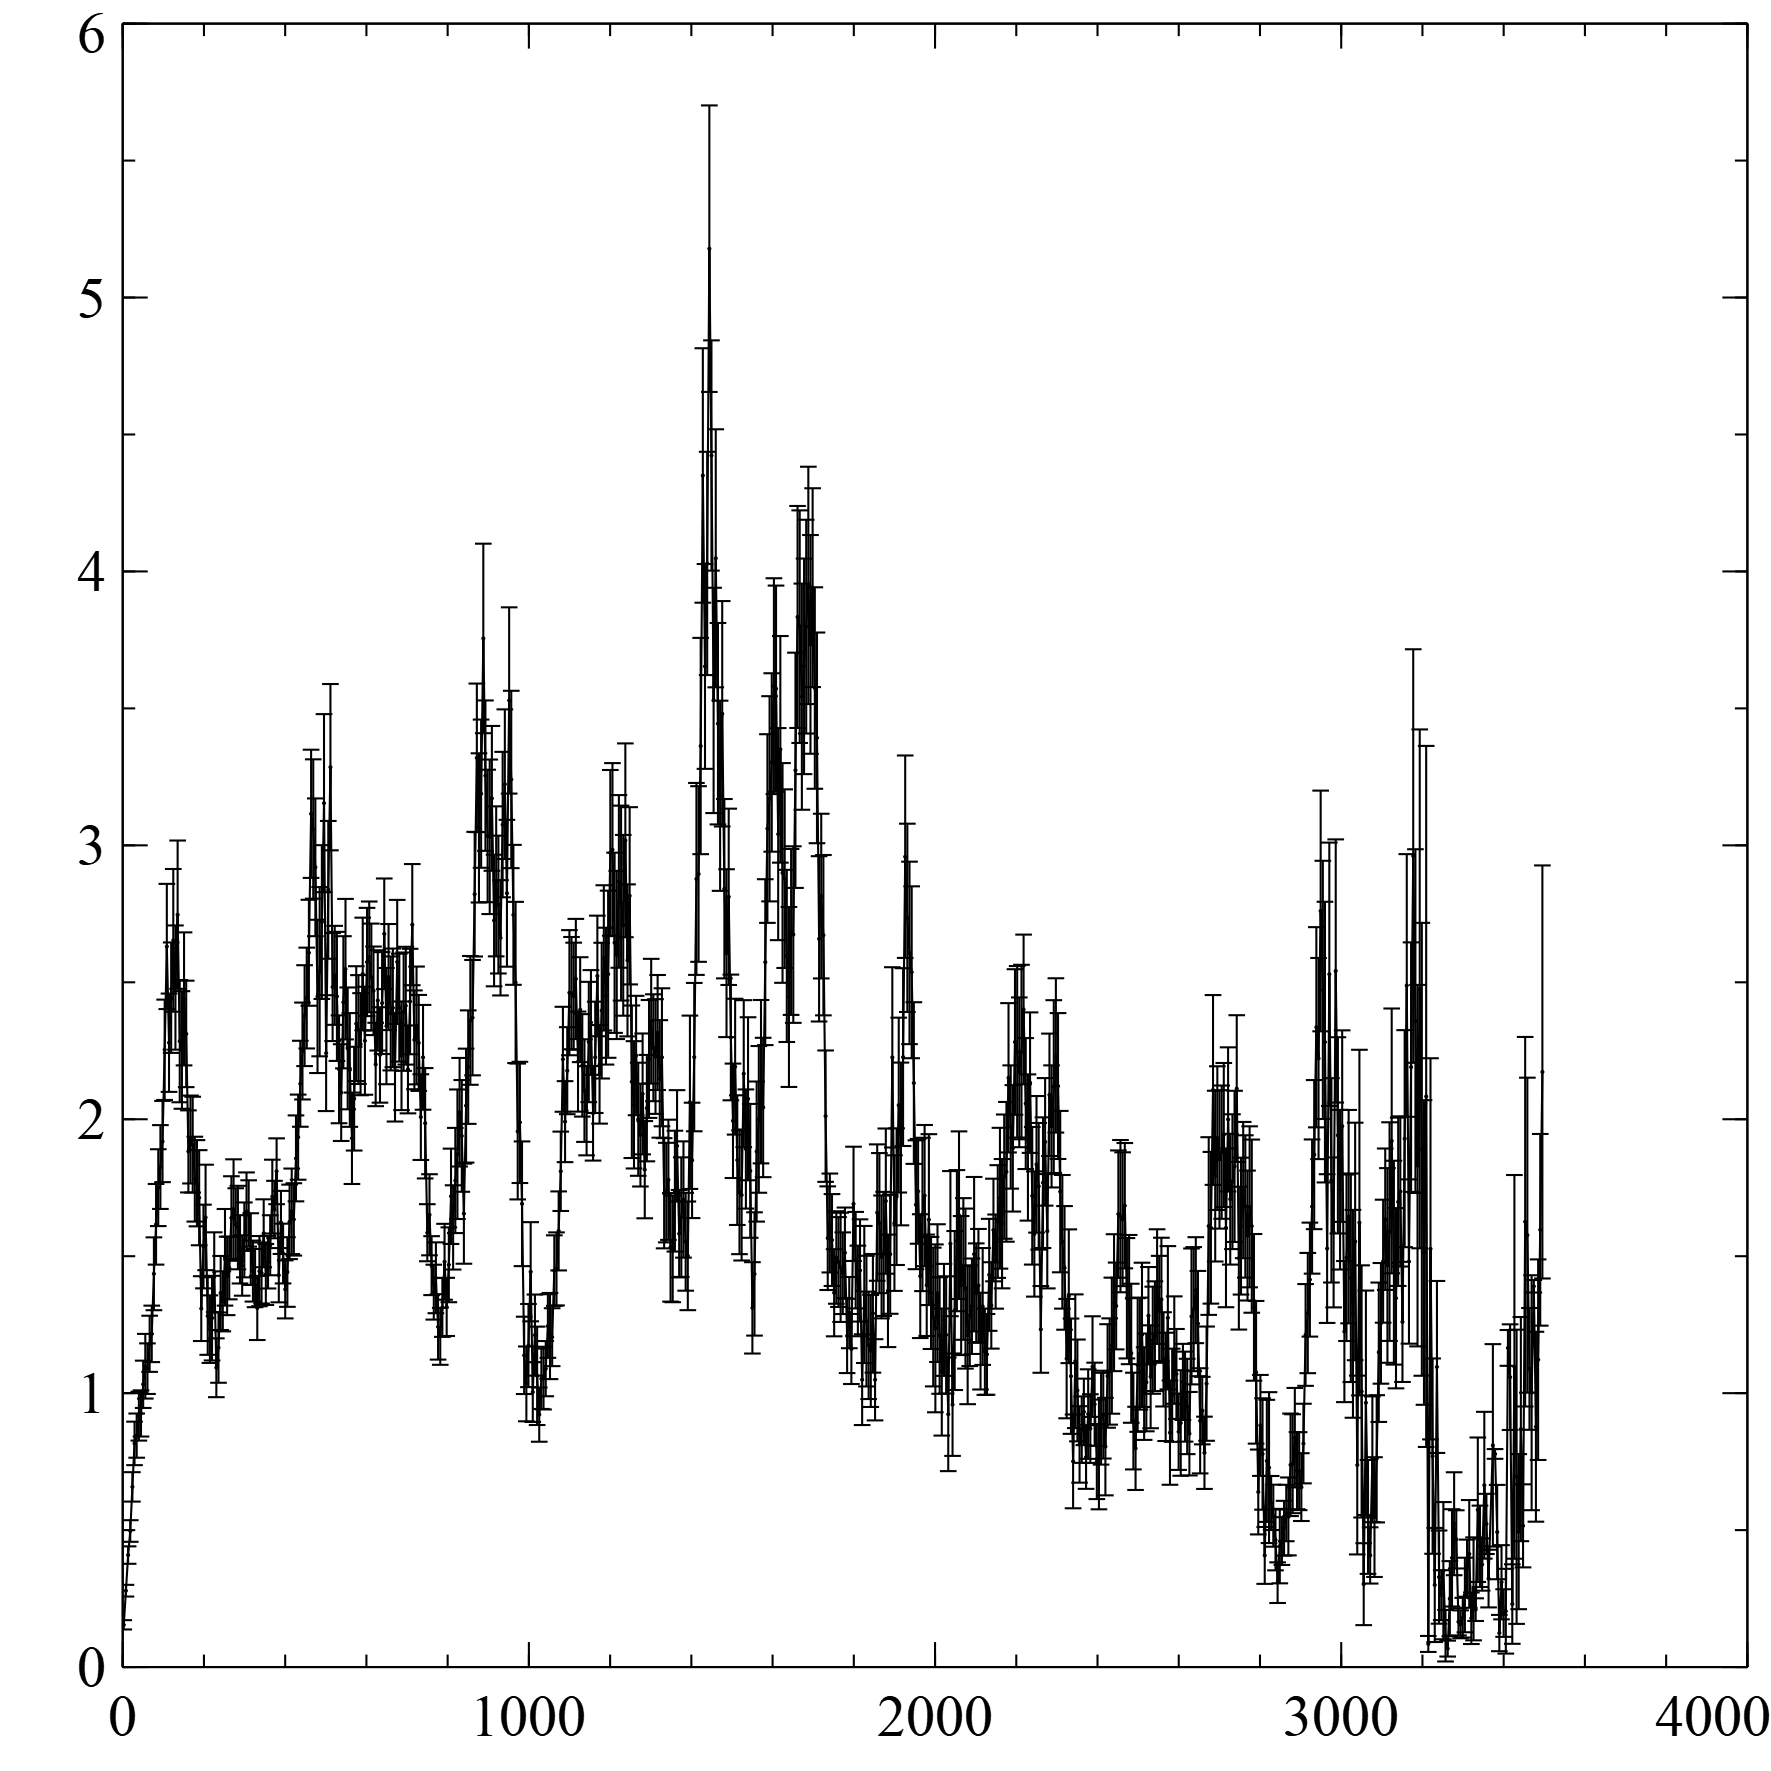
\includegraphics[width=0.8\linewidth]{structureFunctionShape}
		\caption{An example of a structure function with normal scaled axes.(To be replaced)}
		\label{fig:structureFunctionShape}
	\end{minipage}
	\begin{minipage}{0.1\textwidth}
	\end{minipage}
	\begin{minipage}{0.45\textwidth}
		\centering
		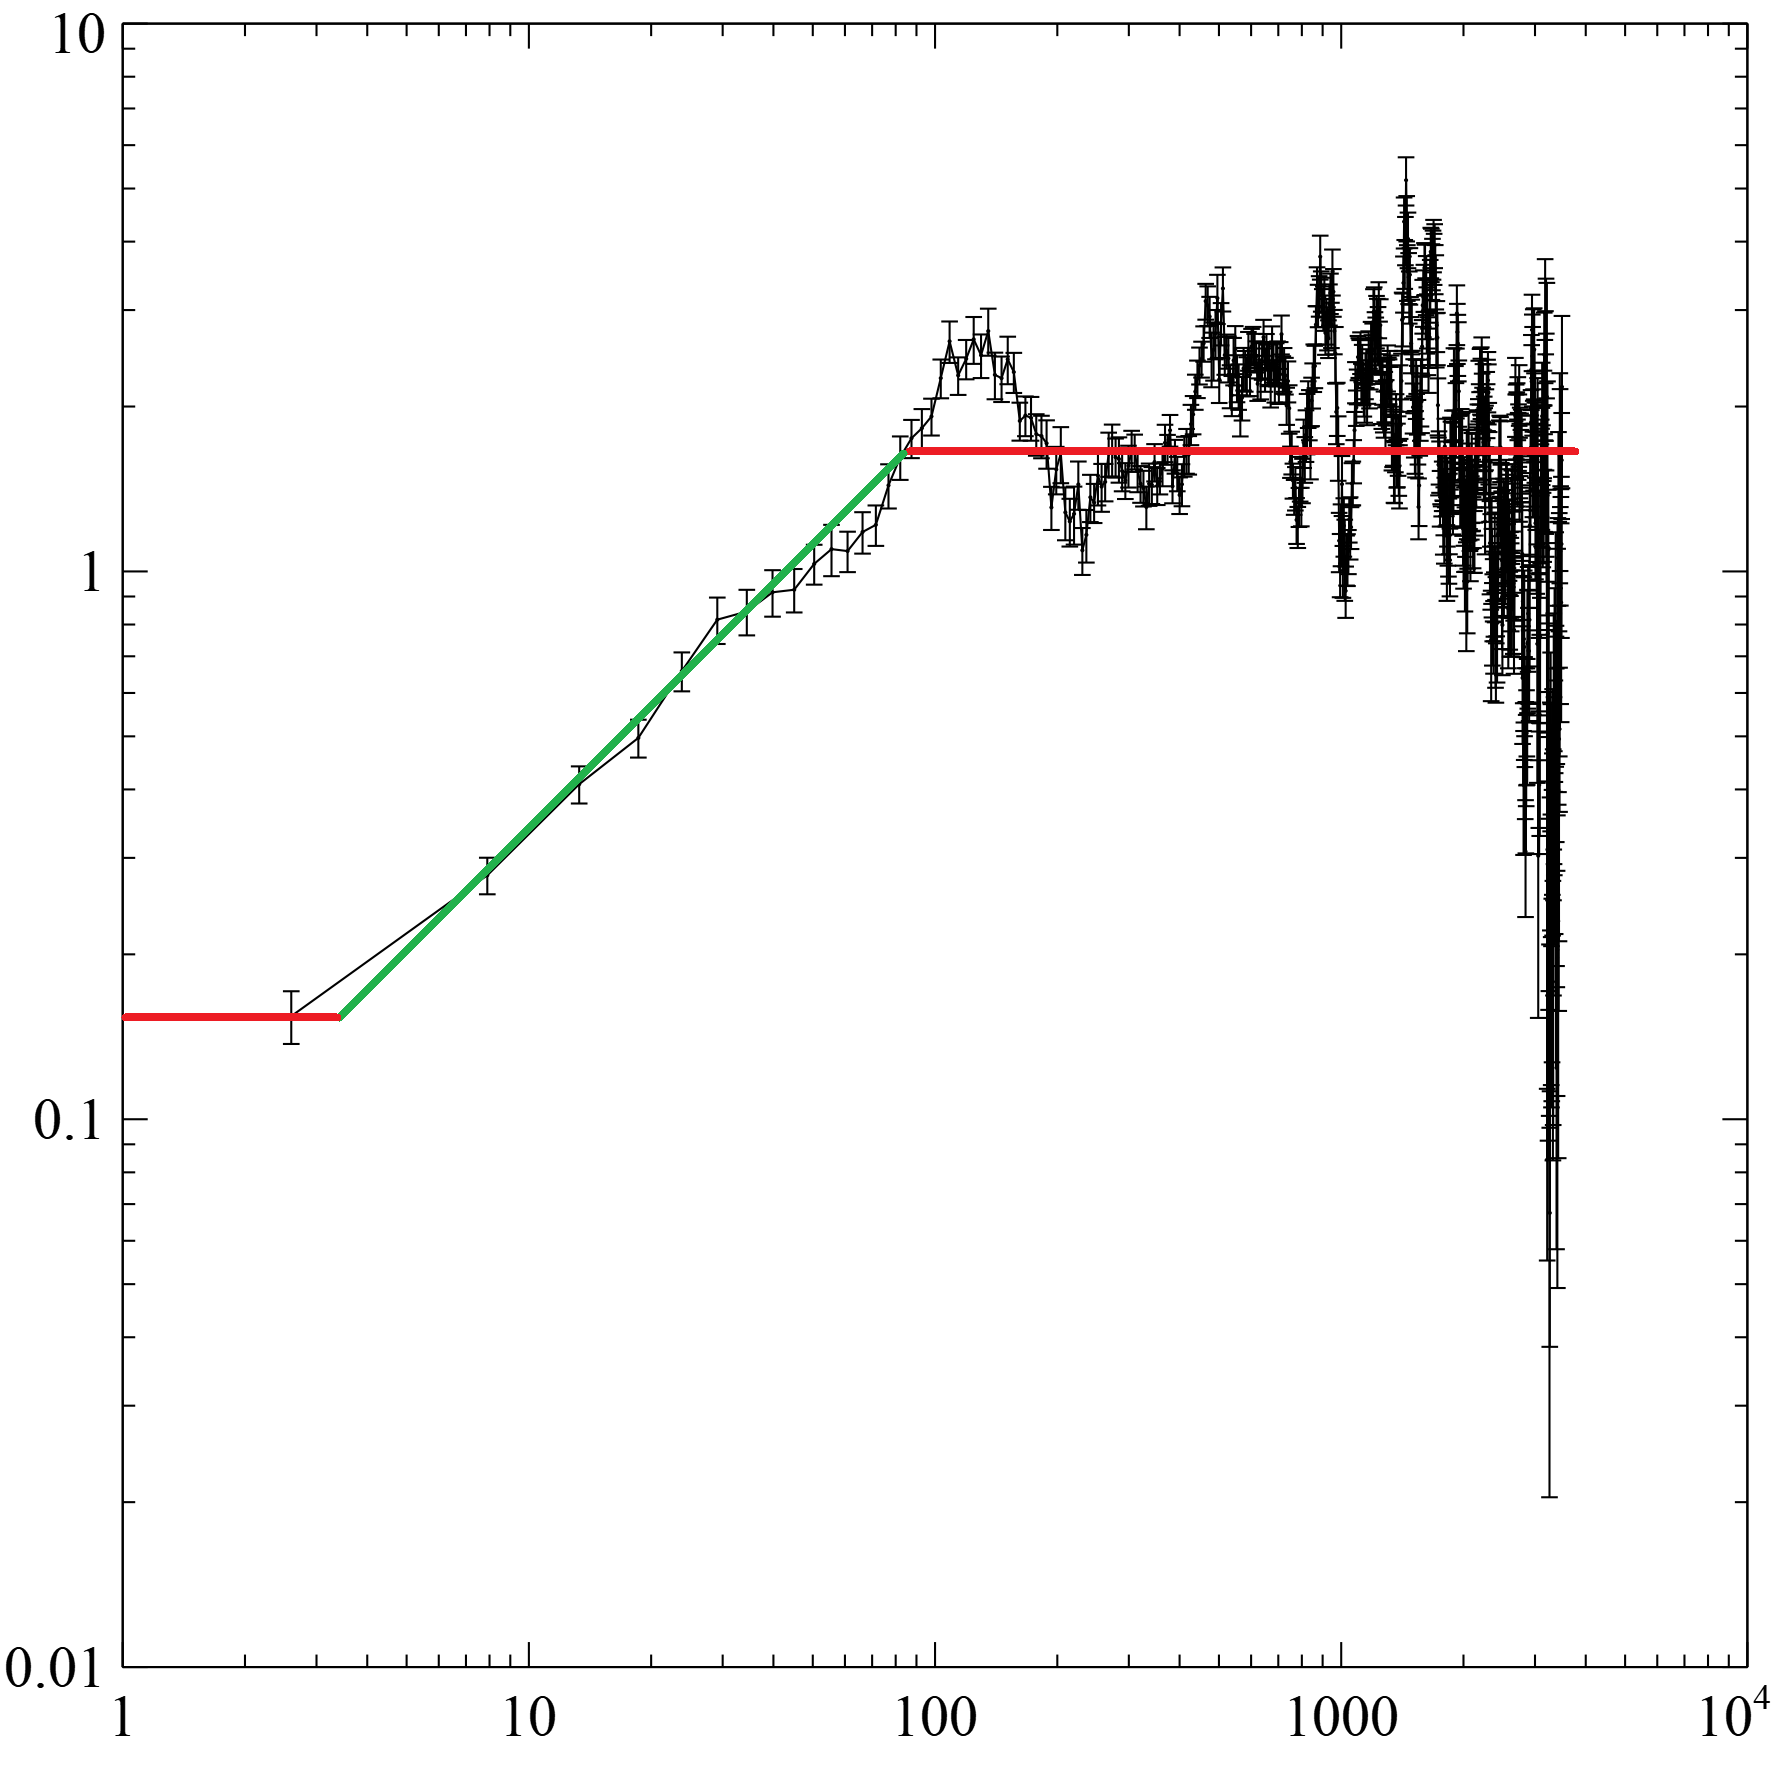
\includegraphics[width=0.8\linewidth]{structureFunctionLogShape}
		\caption{An example of a structure function with log scaled axes. (To be replaced)}
		\label{fig:structureFunctionLogShape}
	\end{minipage}
\end{figure}

Structure functions have a very distinct shape, resembling a sigmoid but dominated by twice the signal variance, $2\sigma^{2}$, on short timescales and twice the noise variance, $2\sigma_{noise}^{2}$, on long timescales. This results in two noise dominated plateaus connected by a power-law section as shown in figure \ref{fig:structureFunctionLogShape}\footnote{\cite{galloblue}} where the plateaus are shown with a red line and the power-law section is shown with a green line overlaid on top of real data for a structure function. As is evident in figure \ref{fig:structureFunctionLogShape}, the upper plateau, corresponding to longer timescales, is completely noise dominated. It is important to note that the axes are log scaled when looking at structure functions as otherwise the resemble Figure \ref{fig:structureFunctionShape}\footnote{\cite{galloblue}}. This brings out the power law section and allows us to fit the structure functions to determine characteristic timescales.

The power-law region of the structure function exists where $\tau_{min}\lesssim\tau\lesssim\tau_{max}$. When $\tau_{max}\ll T$, where $T$ is the total duration of the time-series, we can approximate $\tau_{max}$ to a characteristic timescale, $\tau_{char}$, determined by fundamental source characteristics such as mass, size, matter propagation and others depending on the source of the time-series.

\subsection{\sc Problems and Pitfalls} \label{problemsAndPitfalls}

\begin{figure}[H]
	\centering
	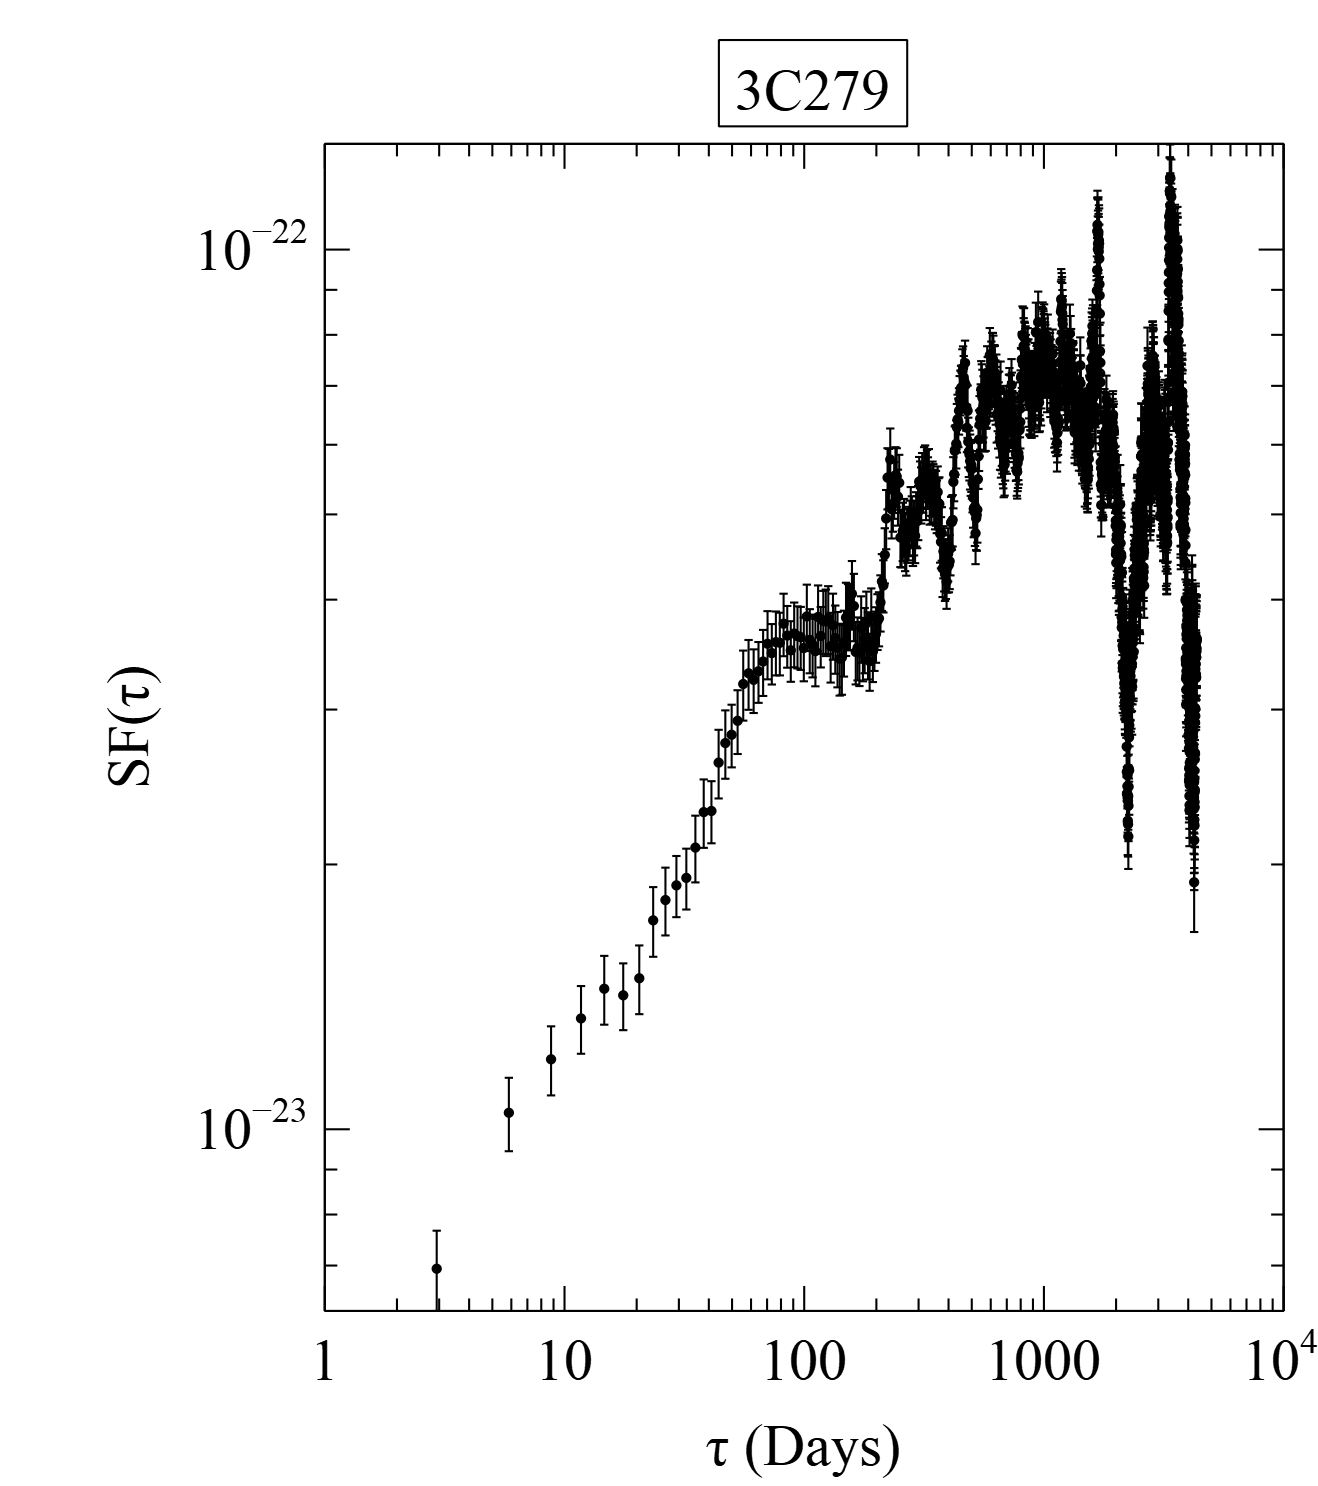
\includegraphics[width=0.6\linewidth]{3C279structurefunction}
	\caption{Structure function for 3C 279 obtained from \cite{rxtepaper}}
	\label{fig:3c279sf}
\end{figure}

The structure functions is an extremely valuable tool for analyzing data that has odd or uneven sampling rates, but it is not without fault. Some things to be aware of when using a structure function on data are as follows. Linear trends that span the entire time-series will artificially steepen the structure function. This can be avoided by removing a best-fit linear model applied to the entire time-series. Some object may have more than one characteristic timescale and this may manifest itself as a third plateau breaking the power-law region in two, as can be seen in Figure \ref{fig:3c279sf}.

\section{\sc SFA usage and description} \label{usageDescription}

SFA is a program written in \verb|C++| to compute the first order structure function of a given set of astronomical time-series data, though it could be used with any set of time-series-like data. As SFA was developed in a Linux environment with Linux as the intended target, MacOS and Windows are not officially supported though one could easily build and compile the program from source for either.

\subsection{\sc Usage}

SFA is intended to be used within a shell environment. Once compiled and installed, proper usage of SFA is:
\begin{center}
	\begin{BVerbatim}
	sfa [options] <path>
	\end{BVerbatim}
\end{center}
Where \verb|[options]| is replaced with the options the user wishes to enable and \verb|<path>| is replaced with the path to the input file.

\subsection{\sc Options}

In its current state, version 0.9.4, SFA has only one fully implemented and available option, though others are works in progress. The following is a list of available options for SFA and their functionality, with their current status stated in their descriptions.
\begin{center}
	\begin{BVerbatim}
	[-o, --output <path>]
	\end{BVerbatim}
\end{center}
Sets the desired output file for SFA to deposit the computed structure function. In this argument pairing \verb|<path>| is the path to the desired output file and both \verb|-o| or \verb|--output| can be used to tell SFA that the next argument is the \verb|<path>| to the output file. This output file does not need to exist as SFA will create the file if necessary.
\begin{center}
	\begin{BVerbatim}
	[-d, --delimiter <string>]
	\end{BVerbatim}
\end{center}
Sets the delimiter string used to parse the input data file. In this argument paring \verb|<string>| is the string the user wishes to use as a delimiter when parsing the input file. This can be a single character such as \verb|","| or a string such as \verb|"..."|. This allows SFA to parse various types of delimited files. It is important to note that SFA uses white-space delimiting to parse input files and as of the current version this option is not enabled and is on the list of works in progress.
\begin{center}
	\begin{BVerbatim}
	[-v, --verbose]
	\end{BVerbatim}
\end{center}
This option is used to tell SFA to provide maximal textual output when running. This is useful mostly for debugging purposes but can also be used if calling SFA from within a script and piping its output to file. In this way one can run SFA on multiple files through automation and later check the file SFA output was piped to for success or failure.

\subsection{\sc Installation and Uninstallation}

There are two methods of installation for SFA, \verb|System-Wide| or \verb|User-Specific|. For installation as a binary available to all users on a system it is recommended to use the \verb|System-Wide| installation method, though this method requires the installing user to have administrative privileges, ie \verb|sudo| on Unix-based systems. If the user does not have administrative rights on a system but still needs the SFA program, the \verb|User-Specific| method can be used. In this case the installation will create the \verb|~/.SFA| directory and will place the \verb|sfa| binary file inside. Both installation methods are detailed on the SFA GitHub repository main page and in the \verb|Readme.md| file included with the project. Included in the projects \verb|makefile| are uninstallation methods for each of the install methods, also detailed in the \verb|Readme.md| file and on the GitHub repository main page.

\subsection{\sc Expected Output} \label{expectedOutput}

When using the SFA program, there is generally very little textual output to the terminal it is run within unless the verbose option \verb|[-v, --verbose]| is used. Instead of screen output SFA computes the first order structure function for the data input and outputs it to a file using tab delimiting. SFA outputs the binned structure function values to the following columns without headers, column 1 is the $\tau$ value, column 2 is the $SF(\tau)$ value, and column 3 is the error in $SF(\tau)$. If no output file is given using the \verb|[-o, --output <path>]| option, then SFA will output the structure function to the file \verb|"[input-file]-[date].out"| where \verb|[input-file]| is the name of the input file given without the file extension and \verb|[date]| is the date when SFA was run on the input file.

\section{\sc Programming SFA} \label{programmingSFA}

 SFA was originally prototyped using the python interpreted scripting language however it was then re-written in \verb|C++| to improve performance and reduce run time. in order to avoid writing libraries for simple operations, SFA relies on \verb|C++17| and makes use of the \verb|<filesystem>| library for path and file operations, which requires the \verb|-lstdc++fs| compile flag and gcc 8+, as well as many of the standard libraries.

\subsection{\sc The SFA algorithm} \label{algorithm}

To calculate the structure function on a set of time-series-like data the decision was made to organize the structure function into bins with widths equal to to the calculated resolution. The resolution of the structure function is the averaged temporal sampling, corresponding approximately to the shortest timescales on which any information can be obtained from the data. Once this resolution has been calculated, it determines the bin widths for the structure function, with bins being centered on $\tau_{i}=(i - \frac{1}{2})\delta$ where $\delta$ is the resolution of the structure function. Once the bins have been determined, a map is created using $\tau=t_{j}-t_{i}$ as the key and a \verb|vector<double>| as the value. This allows us to add the square difference of all value pairs sharing a time difference to the same vector. Once the map has been filled from the input data file, it is then iterated over its keys, first checking which bin the key belongs to and then adding the average of its vector to a temporary vector. Once all keys with $\tau$ belonging to the bin have added the average of their respective vectors to the temporary vector, the average of the temporary vector is then added to a final map representing the structure function with $\tau_{i}$ as its key and $SF(\tau_{i})$ as the value. This final map representing the structure function is then written to a tab delimited file without headers.

\subsection{\sc Cost and Complexity} \label{costComplexity}

Calculating the cost and complexity of SFA is dependent upon a couple of input parameters. Since the number of command line arguments for SFA is at a maximum 6, the domination factor for the complexity of SFA is the number of rows of data, $n$, of the input file. For an input data file of size $n$, the dominating functions for the complexity of SFA are the loading function within the \verb|Lightcurve| class, which has order $O(n)$, and the actual structure function algorithm contained in the \verb|StructureFunction| class. The \verb|StructureFunction| class has a cost of order $O(n)$ in its construction that comes from the calculation of the resolution of the data. In the algorithm for calculating the structure function itself, SFA has a worst-case complexity of $O(n^{3})$ and a best case complexity of $O(n^{2})$.

\chapter{\sc Results and Conclusions} \label{resultsConclusions}

\section{\sc The Data} \label{theData}

Data used for this project was obtained from the \textit{RXTE AGN Timing \& Spectral Database}, \cite{rxtepaper}. The sources were chosen based on the number of data points in the overall light curve as well as the variability in the light curve as determine "by-eye". The sources chosen were 3C 273, 3C 279, Fairall 9, Mkn 79, Mkn 110, and NGC 4051. Observation properties such as the number of data points, start and end dates, etc, can be seen in Table \ref{tab:sourcelist}. 

\begin{minipage}{\linewidth}
	\centering
	\captionof{table}{Source List}\label{tab:sourcelist}
	\resizebox{\textwidth}{!}{
		\begin{tabular}{@{}ccccccccc@{}}
			\toprule
			Source & Type & R.A. & Decl. & Redshift & Start (MDJ) & End (MJD) & Good ObsIDs \\
			\midrule\midrule
			3C 273 & FSRQ & 12 29 06.70 & +02 03 08.6 & 0.1583 & 50115.06 & 55926.56 & 1960 \\
			3C 279 & FSRQ & 12 56 11.1 & -05 47 22 & 0.5326 & 50104.63 & 55925.99 & 1987 \\
			Fairall 9 & Sy1 & 01 23 45.78 & -58 48 20.8 & 0.0470 & 50390.61 & 52699.51 & 707 \\
			Mkn 79 & Sy1.2 & 07 21 53.45 & +49 48 34.7 & 0.0222 & 51610.57 & 55925.58 & 1646 \\
			Mkn 110 & NLSy1.5 & 09 25 12.87 & +52 17 10.5 & 0.0353 & 51610.56 & 55925.59 & 1432 \\
			NGC 4051 & NLSy1.5 & 12 03 09.61 & +44 31 52.8 & 0.0023 & 501996.49 & 55925.45 & 2125 \\
			\bottomrule
		\end{tabular}
	}\par
	\bigskip
	Data taken from \textit{RXTE AGN Timing \& Spectral Database}
\end{minipage}

\begin{figure}[H]
	\centering
	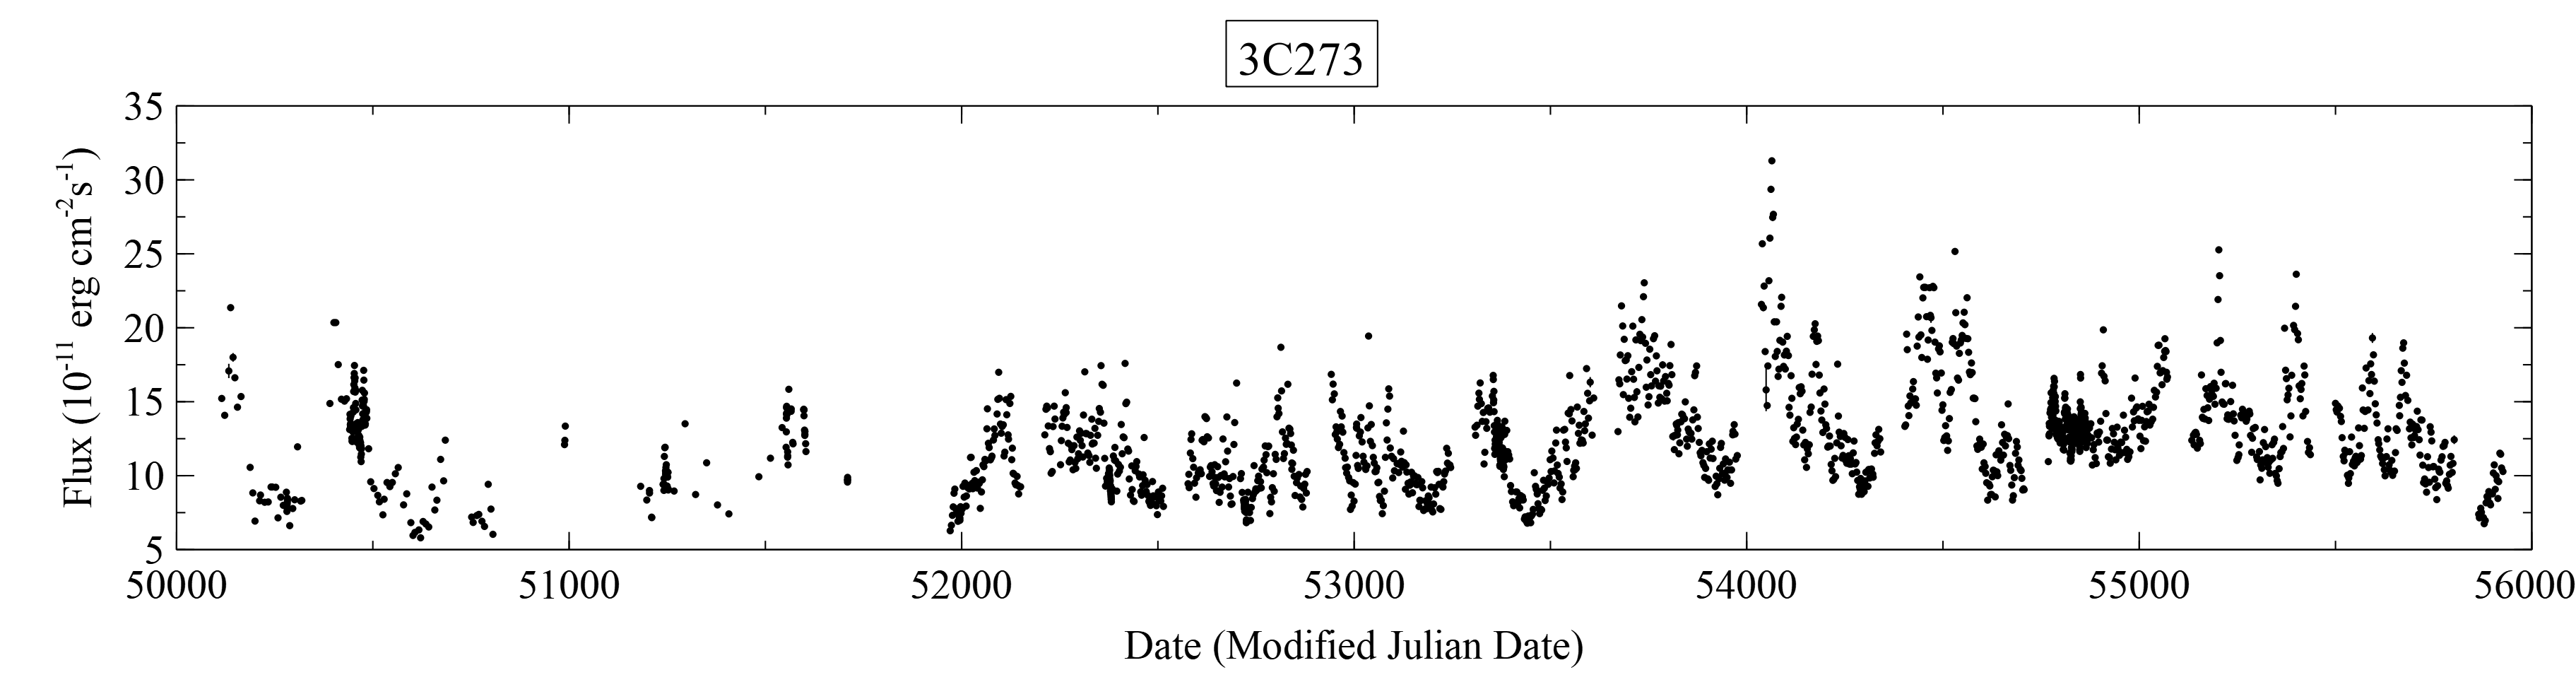
\includegraphics[width=\linewidth]{3C273lightcurve}
	\caption{Light curve for 3C 273}
	\label{fig:3c273lc}
\end{figure}

\begin{figure}[H]
\centering
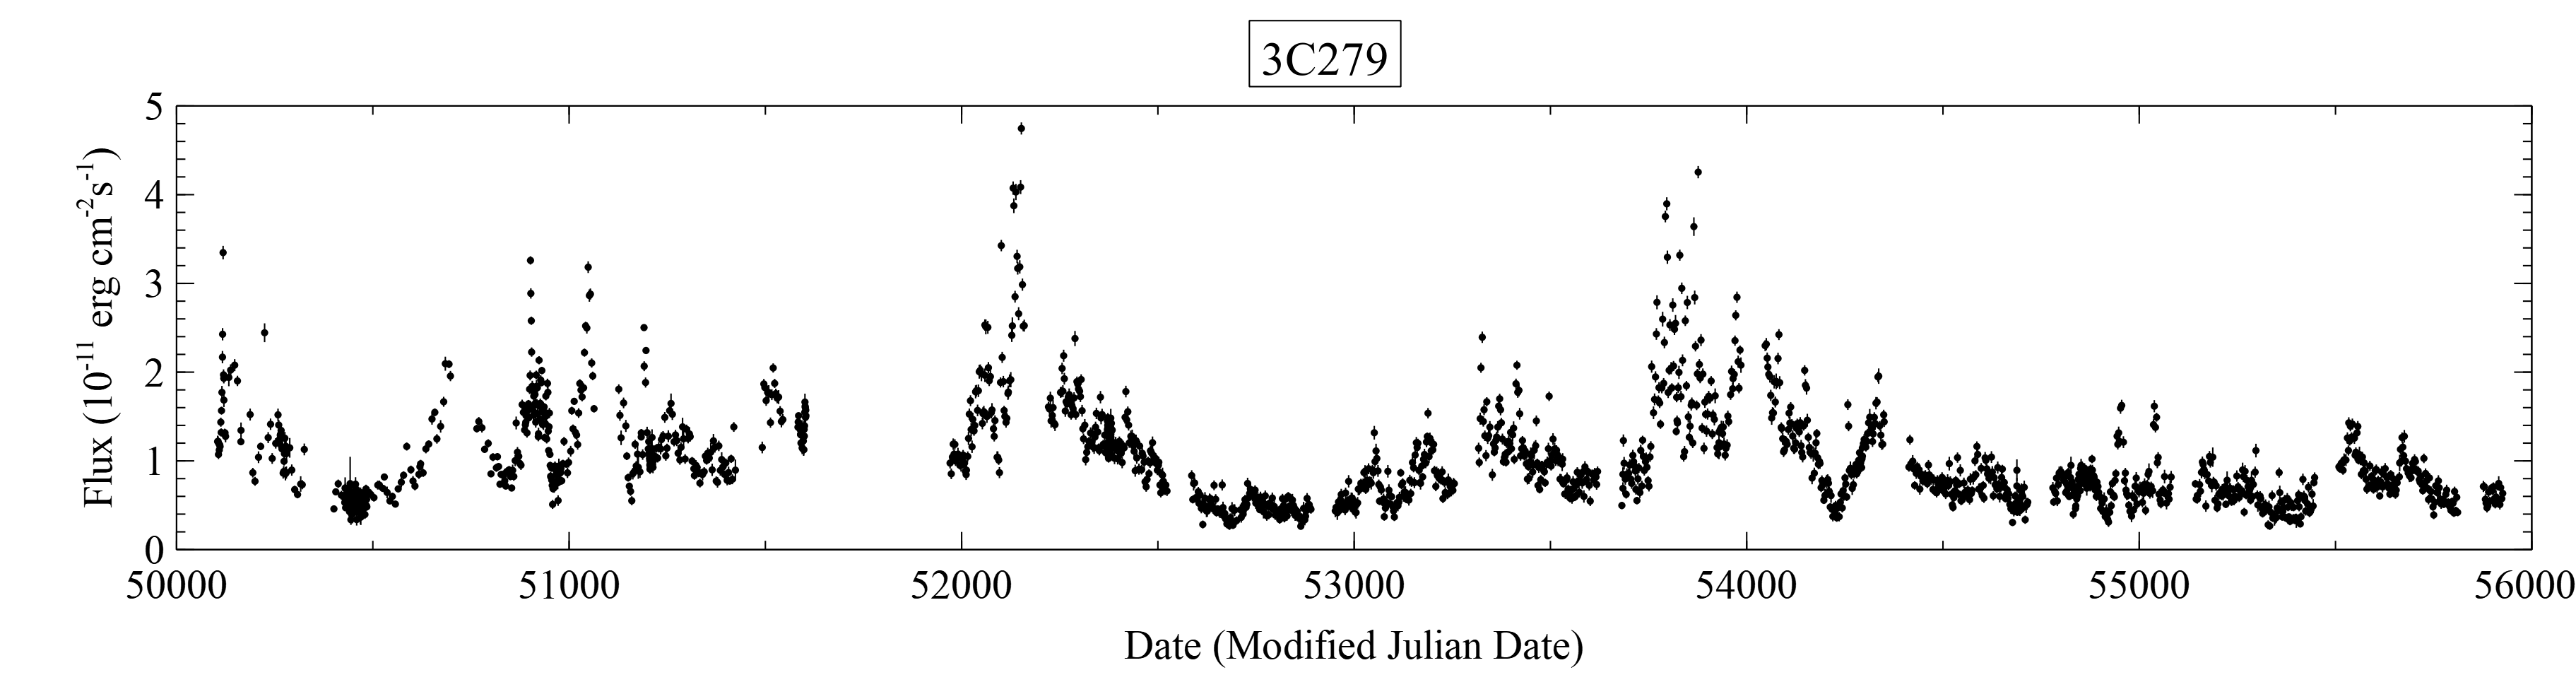
\includegraphics[width=\linewidth]{3C279lightcurve}
\caption{Light curve for 3C 279}
\label{fig:3c279lc}
\end{figure}

\begin{figure}[H]
\centering
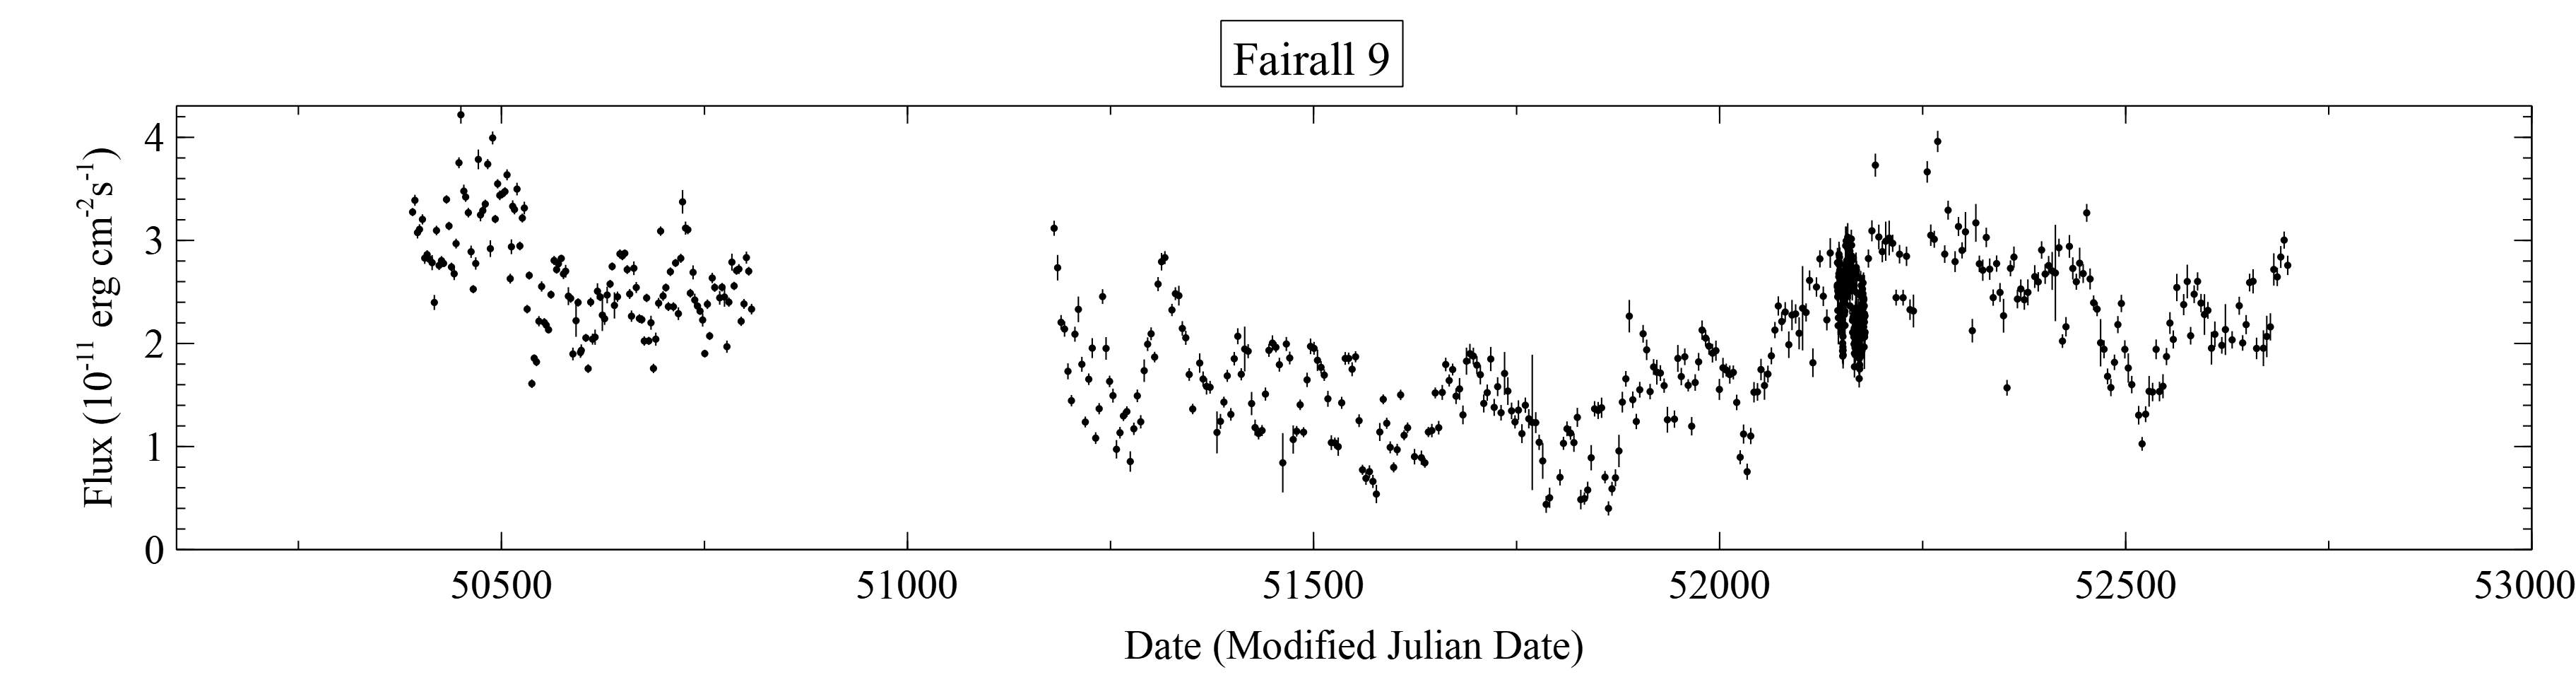
\includegraphics[width=\linewidth]{Fairall9lightcurve}
\caption{Light curve for Fairall 9}
\label{fig:fairall9lc}
\end{figure}

\begin{figure}[H]
\centering
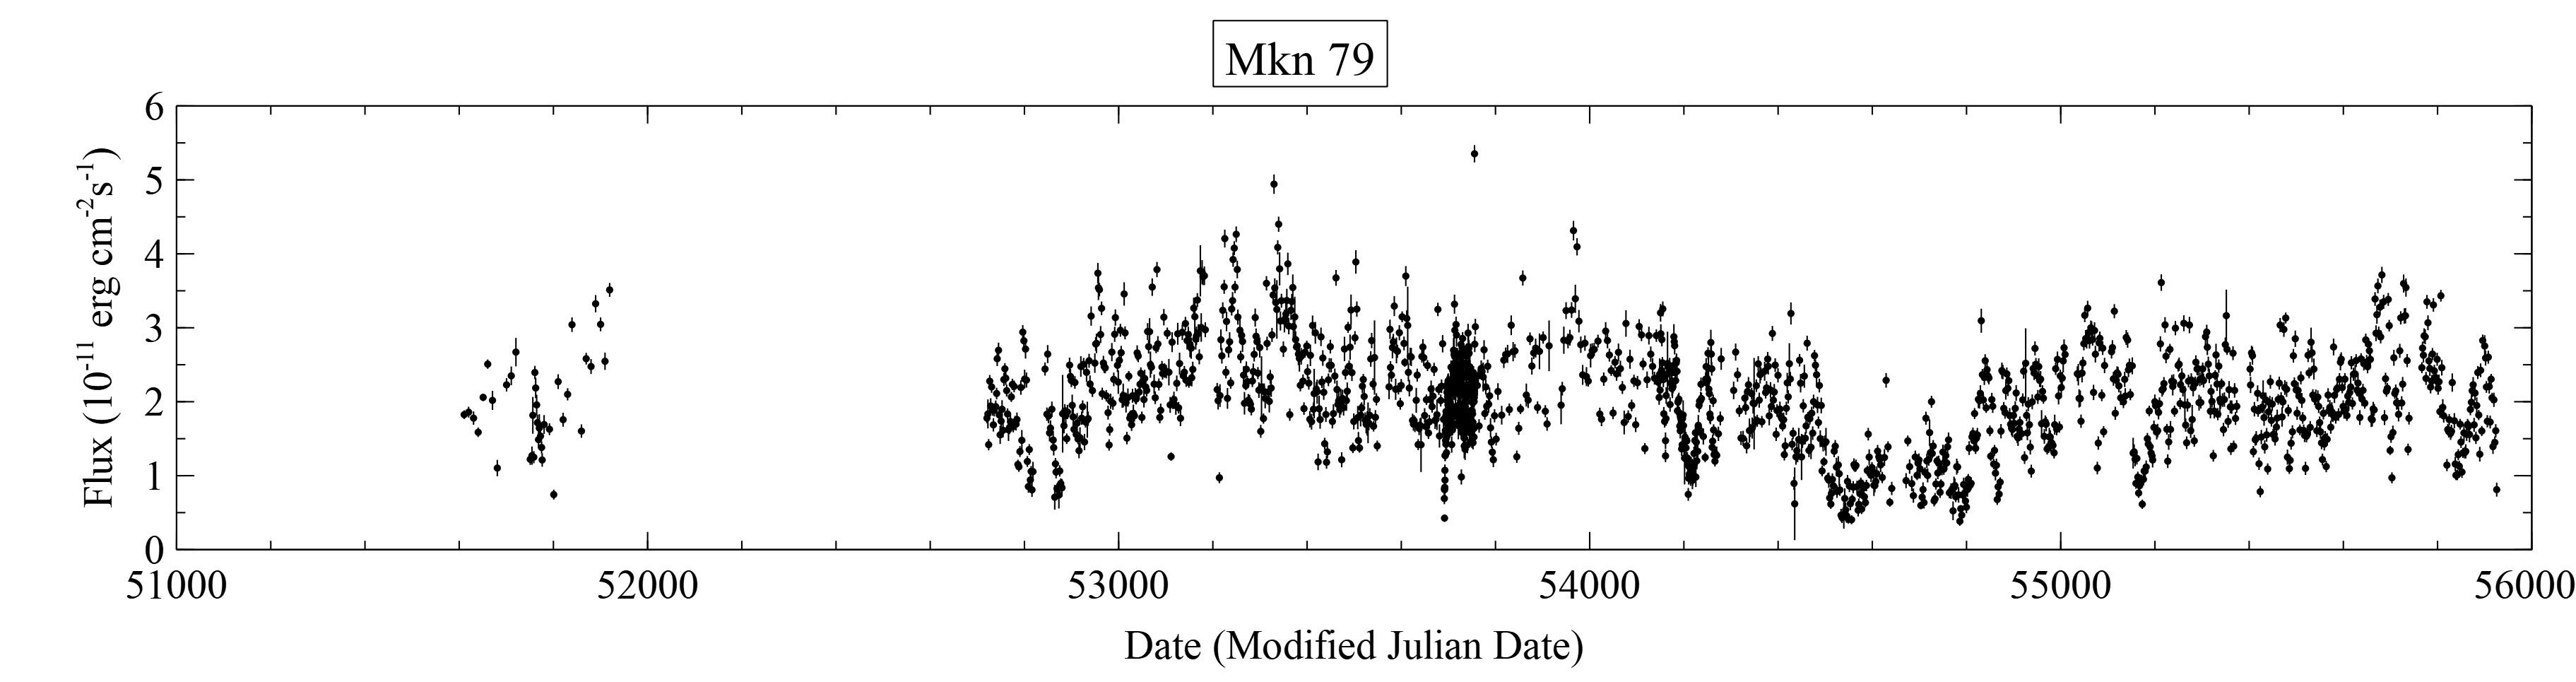
\includegraphics[width=\linewidth]{Mkn79lightcurve}
\caption{Light curve for Mkn 79}
\label{fig:mkn79lc}
\end{figure}

\begin{figure}[H]
\centering
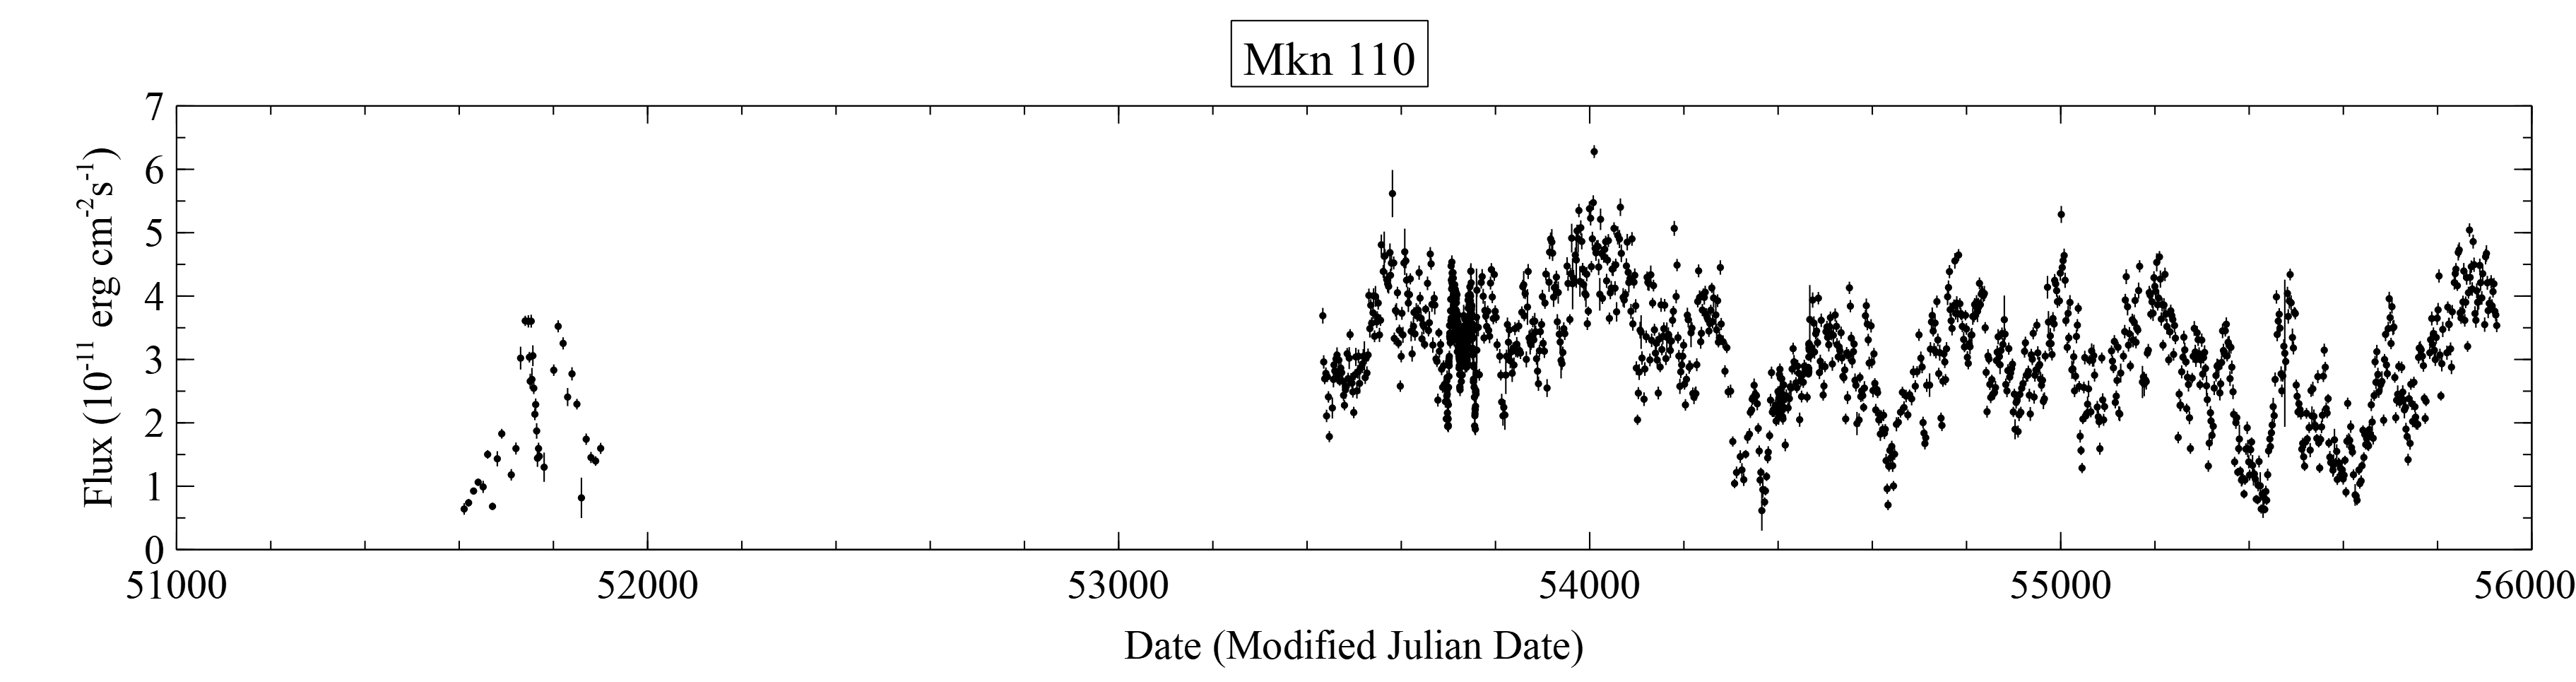
\includegraphics[width=\linewidth]{Mkn110lightcurve}
\caption{Light curve for Mkn 110}
\label{fig:mkn110lc}
\end{figure}

\begin{figure}[H]
\centering
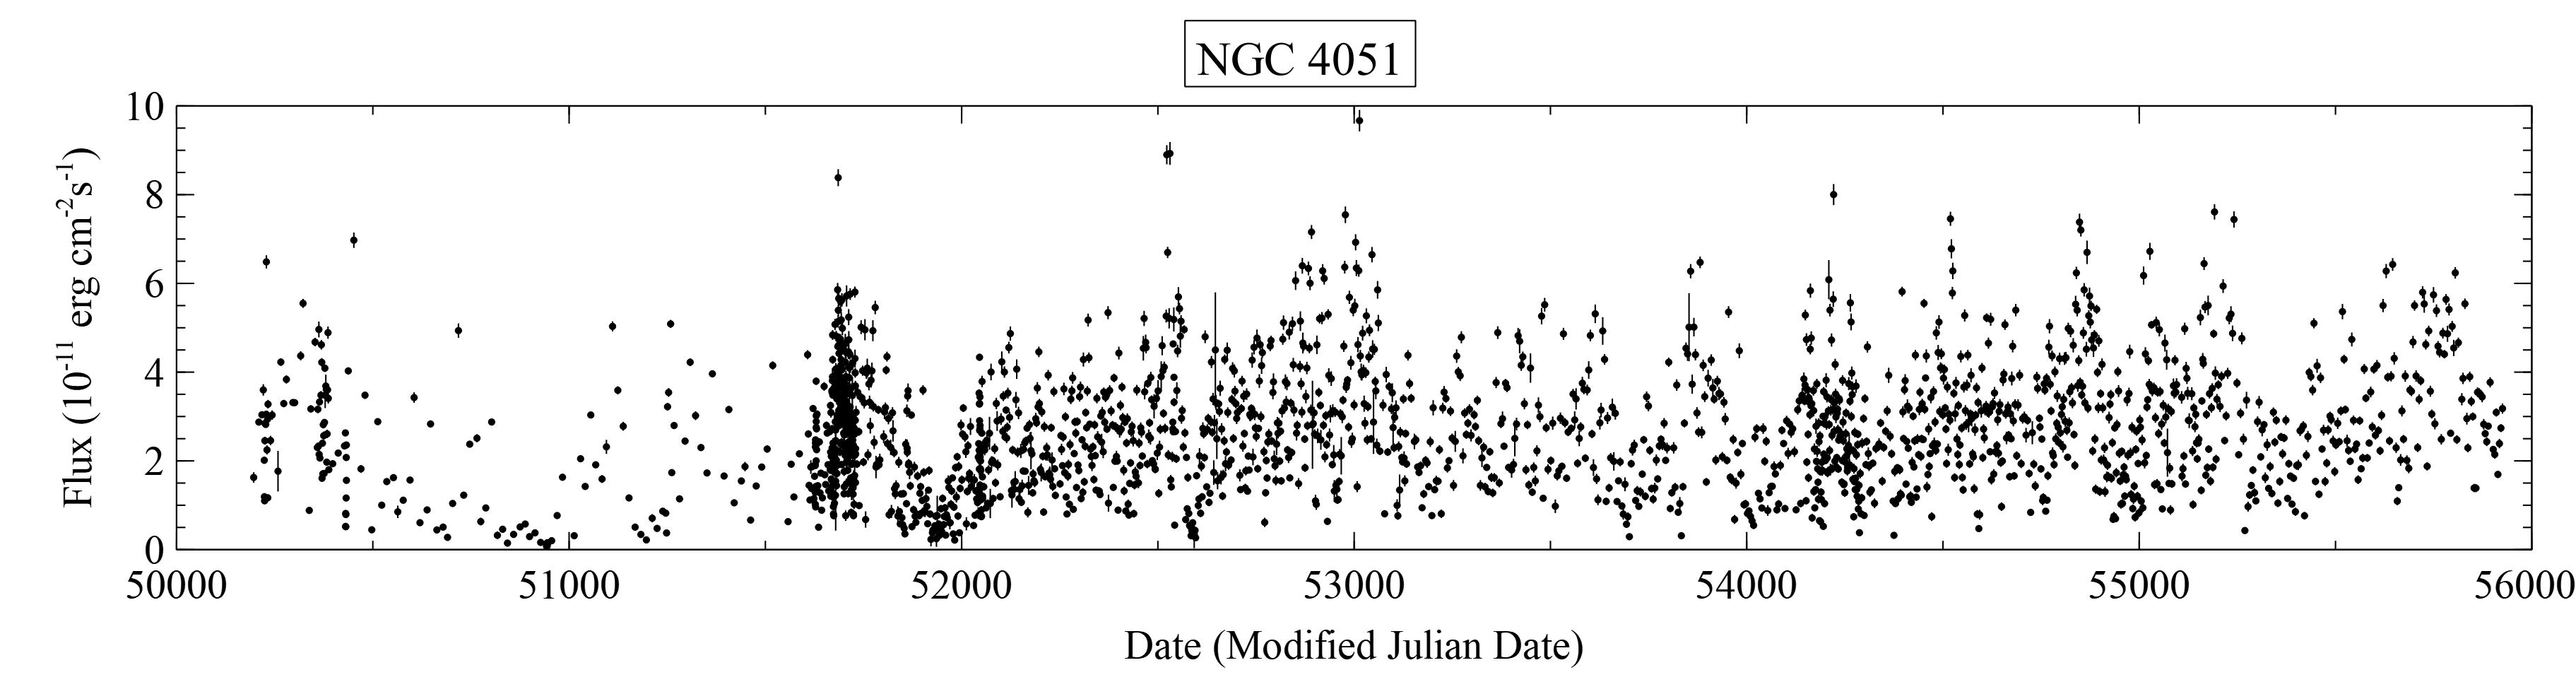
\includegraphics[width=\linewidth]{NGC4051lightcurve}
\caption{Light curve for NGC 4051}
\label{fig:ngc4051lc}
\end{figure}

\section{\sc Results} \label{results}

A review of the results of running SFA on observational data

\begin{figure}[H]
	\centering
	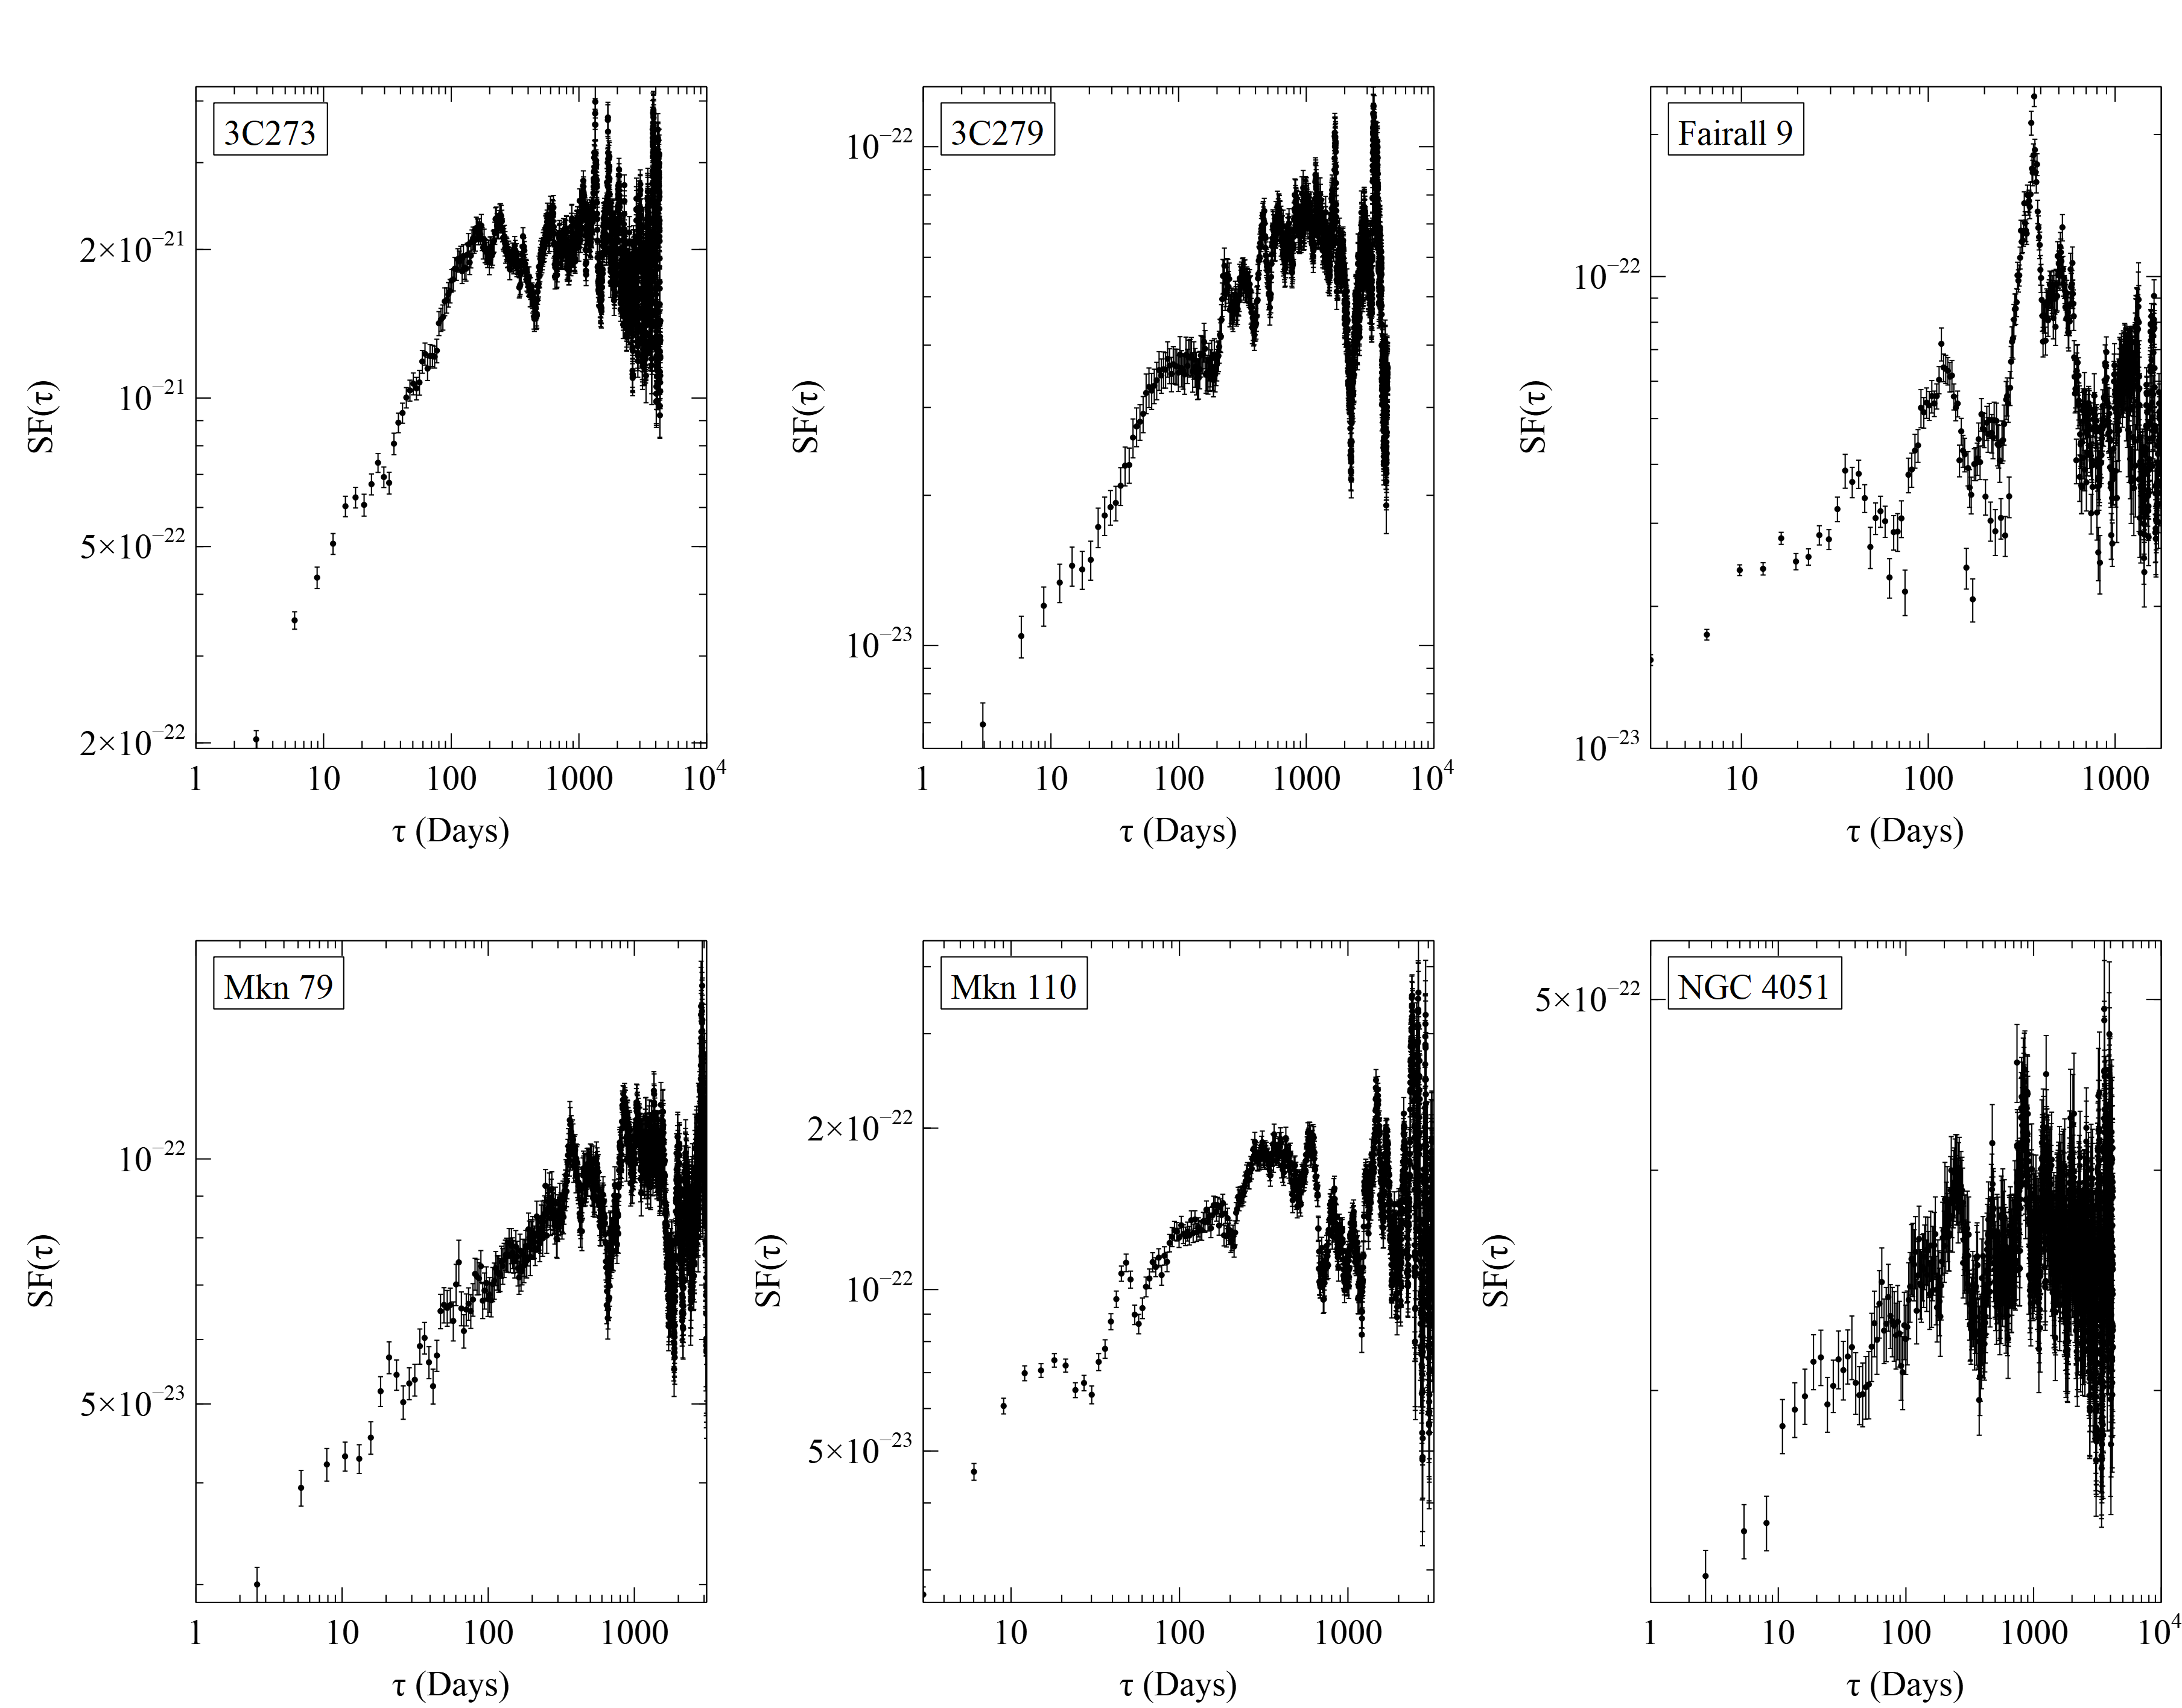
\includegraphics[width=\linewidth]{combinedstructurefunctions}
	\caption{Structure functions for 3C 273, 3C 279, Fairall 9, Mkn 79, Mkn 110, and NGC 4051}
	\label{fig:combosf}
\end{figure}

\section{\sc Conclusions} \label{conclusions}

Theoretical conclusions based on the findings of SFA

\chapter{\sc Future Work} \label{futureWork}

Potential future work and applications of SFA


\appendix

\chapter{Structure Function} \label{appendixSFA}
\label{app:sfa}
If you wanted an appendix, it would go in like this.  It would be 
referenced using Appendix~\ref{app:sfa}.


\begin{singlespace}
\bibliography{SMU-HonorsThesis-template}
\end{singlespace}
\end{document}
